%\documentclass[PhD]{iitmdiss}
%\documentclass[MS]{iitmdiss}
%\documentclass[MTech]{iitmdiss}
\documentclass[hidelinks,BTech]{iitmdiss}
\usepackage{times}
\usepackage{t1enc}
\usepackage{graphicx}
\usepackage{epstopdf}
\usepackage{hyperref} % hyperlinks for references.
\usepackage{amsmath} % easier math formulae, align, subequations \ldots
\usepackage{xcolor}
\usepackage{amsfonts}
\usepackage{subcaption}
\usepackage{float}

\newcommand\todo[1]{\textcolor{red}{{\bf TODO}: #1}}

\begin{document}


%%%%%%%%%%%%%%%%%%%%%%%%%%%%%%%%%%%%%%%%%%%%%%%%%%%%%%%%%%%%%%%%%%%%%%
% Title page

\title{Autonomous control of Quad-rotor and payloads using Reinforcement Learning}

\author{Abdeali J. Kothari}

\date{April 2016}
\department{PHYSICS}

%\nocite{*}
\maketitle

%%%%%%%%%%%%%%%%%%%%%%%%%%%%%%%%%%%%%%%%%%%%%%%%%%%%%%%%%%%%%%%%%%%%%%
% Certificate
\certificate

\vspace*{0.5in}

\noindent This is to certify that this thesis, submitted by {\bf Abdeali J. Kothari}, to the Indian Institute of Technology, Madras, for the award of the degree of {\bf B. Tech.}, is a bona fide record of the research work done by them under our supervision. The contents of this thesis, in full or in parts, have not been submitted to any other Institute or University for the award of any degree or diploma.

\vspace*{1.5in}

\begin{singlespacing}

\begin{minipage}[t]{0.45\textwidth}
  {\bf Prof. Balaraman Ravindran} \\
  Research Guide \\
  Associate Professor \\
  Dept. of Computer Science \\
  and Engineering \\
  IIT-Madras, 600 036
\end{minipage}
\hfill
\begin{minipage}[t]{0.45\textwidth}
  {\bf Prof. Ramkrishna Pasumarthy} \\
  Research Guide \\
  Assistant Professor \\
  Dept. of Electrical Engineering \\
  IIT-Madras, 600 036
\end{minipage}

\end{singlespacing}

\vspace*{0.25in}
\noindent Place: Chennai\\
Date: \todo{4 April 2016}


%%%%%%%%%%%%%%%%%%%%%%%%%%%%%%%%%%%%%%%%%%%%%%%%%%%%%%%%%%%%%%%%%%%%%%
% Acknowledgements
\acknowledgements

I would like to thank my university Indian Institute of Technology, Madras for giving me the opportunity to work on this project. My guides for allowing me to work with them and their invaluable help throughout the project, right from the identification of the project topic to helping mould approaches and identifying new directions to work in when a line of thought had to be abandoned.

I'd also like to thank Kunal Grover (ME12B033) who has worked with me during the project. With various intriguing conversations on concept ideas, planning, learning methodologies, coding practices, and simulation design it's been great working with him.

%%%%%%%%%%%%%%%%%%%%%%%%%%%%%%%%%%%%%%%%%%%%%%%%%%%%%%%%%%%%%%%%%%%%%%
% Abstract

\abstract

\noindent KEYWORDS: \hspace*{0.5em} \parbox[t]{4.4in}{Quad-rotor Control; Payload control; Reinforcement Learning; Policy Search; PEGASUS.}

\vspace*{24pt}

\noindent Autonomous quad-rotor flight is a problem which is challenging because of the complex dynamics and noise involved. A method to control quad-rotors is described by applying policy search from reinforcement learning. First a simulation is set-up training the quad-rotor using gazebo and ROS. The simulated model is used to learn position control like hovering in place, moving to a specific location, and also controlling the final yaw. Once a stable position control is achieved the quad-rotor learns to move in various trajectories and paths using a trajectory control technique. Finally, a payload is attached to the quad-rotor and the quad-rotor learns to move the payload using position and trajectory control.

\pagebreak

%%%%%%%%%%%%%%%%%%%%%%%%%%%%%%%%%%%%%%%%%%%%%%%%%%%%%%%%%%%%%%%%%
% Table of contents etc.

\begin{singlespace}
\clearpage
\phantomsection
\addcontentsline{toc}{chapter}{TABLE OF CONTENTS}
\tableofcontents
% \thispagestyle{empty}

% \listoftables
% \addcontentsline{toc}{chapter}{LIST OF TABLES}

\listoffigures
\addcontentsline{toc}{chapter}{LIST OF FIGURES}
\end{singlespace}


%%%%%%%%%%%%%%%%%%%%%%%%%%%%%%%%%%%%%%%%%%%%%%%%%%%%%%%%%%%%%%%%%%%%%%
% Abbreviations
% \abbreviations

% \noindent
% \begin{tabbing}
% xxxxxxxxxxx \= xxxxxxxxxxxxxxxxxxxxxxxxxxxxxxxxxxxxxxxxxxxxxxxx \kill
% \textbf{IITM}   \> Indian Institute of Technology, Madras \\
% \textbf{RTFM} \> Read the Fine Manual \\
% \end{tabbing}

% \pagebreak

%%%%%%%%%%%%%%%%%%%%%%%%%%%%%%%%%%%%%%%%%%%%%%%%%%%%%%%%%%%%%%%%%%%%%%
% Notation

% \chapter*{\centerline{NOTATION}}
% \addcontentsline{toc}{chapter}{NOTATION}

% \begin{singlespace}
% \begin{tabbing}
% xxxxxxxxxxx \= xxxxxxxxxxxxxxxxxxxxxxxxxxxxxxxxxxxxxxxxxxxxxxxx \kill
% \textbf{$r$}  \> Radius, $m$ \\
% \textbf{$\alpha$}  \> Angle of thesis in degrees \\
% \textbf{$\beta$}   \> Flight path in degrees \\
% \end{tabbing}
% \end{singlespace}

% \pagebreak
\clearpage

% The main text will follow from this point so set the page numbering
% to arabic from here on.
\pagenumbering{arabic}


%%%%%%%%%%%%%%%%%%%%%%%%%%%%%%%%%%%%%%%%%%%%%%%%%%
% Introduction.

\chapter{Introduction}

\section{Motivation}

In robotics, there are many cases where the problem to solve is not known, is stochastic, has non-linear dynamics and has a large number of actions and states. In such cases, traditional control methods which require complete knowledge of the system may be difficult to model. Reinforcement learning is a method by which the robot does not need much knowledge about the environment, and can be used in such cases.

Quad-rotors (or drones) are becoming common with commercial quad-rotors available in the market and are popular among hobbyists. Most commercial quad-rotors are not certified to be operated outside line of sight, let alone autonomously. The major issue for this is the unexpected noise from the environment which cannot be controlled in a real life environment. There has been a lot of research in this domain, and autonomous control of quad-rotors is becoming a reality.

One of the major use cases for an autonomous quad-rotor is to carry payloads from one place to another. This could be used for something as simple as delivery or for reconnaissance. The payloads adds a new complexity and constraints to the earlier system. For example, a payload shouldn't hit obstacles on the course. And if the payload is attached using a non-rigid joint to the quad-rotor, the dynamics become even more complicated.

As a reinforcement problem, this brings up further questions. In the original scenario, it was already difficult to define the reward as a "good flight" is not clearly defined. Now, there is also a need to define a "good flight for the payload".

\begin{figure}[H]
  \centering
    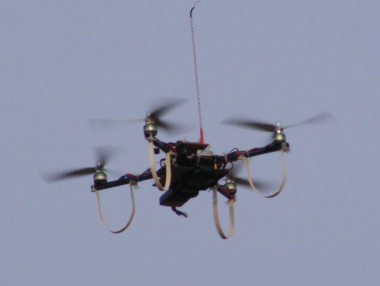
\includegraphics[width=0.5\textwidth]{quadrotor.jpg}
    \caption{Picture of a quad-rotor flying.}
\end{figure}

\section{Outline}

It is difficult to work with quad-rotors without good simulators. In reinforcement learning, where the quad-rotor learns the bad states and good states, collisions, flips, and unstable states are unavoidable. A real quad-rotor would break within a few trials of this learning procedure.

Hence, the first step is to set-up a simulated environment where the quad-rotor can learn. Ideally, the simulated quad-rotor is as close to real as possible so that the learning can be directly transferred. The gazebo simulator was used with ROS to emulate this. This enables us to perform simulate wind, turbulence, motors, and even joints.

Next, a control algorithm which would be suitable for our specific use case with multi-dimensional states and continuous actions and states is needed. PEGASUS (a policy search method) was used to learn the control of the quad-rotor. It is capable of handling the stochastic nature of the environment and the continuous action and state space well. It has already been used to control helicopters and perform stunts with them.

Initially PEGASUS control is used to control the quad-rotor without any payload. Then, a payload is added and a policy is learnt that can control the payload. Once this is done, trajectories are traced using the PEGASUS control with various popular methods. Apprenticeship learning helps in performing special unstable trajectories also.

%%%%%%%%%%%%%%%%%%%%%%%%%%%%%%%%%%%%%%%%%%%%%%%%%%
\chapter{Background}

\section{Reinforcement Learning}

\subsection{Markov Decision Processes}
A common problem in learning is that of an agent learning to act logically in an environment by interacting with it and obtaining feedback of some sort in the form of rewards. The agent and the environment compose a dynamic system. The agent is the part which is controllable (the input) and the environment is that part that cannot be controlled. The agent's objective is to learn a policy to maximize the some function of the rewards it receives from the environment.

A Markov Decision Process \cite{MarkovDecisionProcess} (MDP) is used to model such dynamic systems. MDPs are a general mathematical framework to model decision making in scenarios where some stochasticity is involved and systems that can be partially controlled. The MDP is a tuple with:
\begin{itemize}
\item{{\bf State space ($\mathbb{S}$)} The set of possible states an agent can find itself in.}
\item{{\bf Action space ($\mathbb{A}$)} The set of all actions that an agent can perform.}
\item{{\bf Transition function ($P(s'|s,a)$)} The probability of a transition from one state to another assuming an action has been taken.}
\item{{\bf Reward function ($R(s, a)$)} The reward got from the environment for taking an action $a$ at state $s$.}
\item{{\bf Initial state distribution ($D$)} The distribution from which the initial state $s_0$ is drawn from.}
\item{{\bf Discount factor ($\gamma \in [0,1]$)} The discount factor which specifies how important future rewards are.}
\end{itemize}

\subsection{The Reinforcement learning problem}
Consider a complicated dynamic task like bipedal walking. The agent here is the learner who can control the motions of joints like the knee, and ankle. When the agent uses these controllable actuators, it gets rewards from the environment, like falling down, walking in the wrong direction, and losing balance. Here, the agent does not know what the next state will be nor what the reward it would get for an action when it begins this task.

The agent needs to attempt various actions and observe the state and the reward at every step. Using this observed state, the agent chooses an action and obtains a reward for this action. The next state would depend on the transition function, and once again the agent chooses an action in this new state. The goal of the agent is to find which action should be performed in a state to optimize the cumulative reward (or some function of the set of rewards). This mapping is the policy $\pi$.

Hence the policy is any function denoted by the mapping:
\begin{equation} \begin{split}
  \pi :& \quad \mathbb{S} \rightarrow \mathbb{A} \qquad or \\
  \pi :& \quad \mathbb{S} \times \mathbb{A} \rightarrow [0,1]
\end{split} \end{equation}

\noindent {\bf Difference between Planning and Reinforcement learning}

Planning is the task of fincding an optimal policy for the agent when the agent is given the complete knowledge of the environment. In Reinforcement Learning, the agent is given no knowledge of the environment. The agent must explore, gain experience, and perform actions based on the inferences of the past expereince.

\subsection{Application of Reinforcement Learning}
Reinforcement learning has been applied to a wide variety of spheres ranging from robotics \cite{HelicopterPegasus} to game playing like checkers \cite{RLInCheckers}, the game of Go \cite{RLInGo} and the famous TD-Gammon player \cite{RLInBackgammon}. The game agents were able to beat some of the best players of the time. The gaming agents led to advancements in the theory of backgammon and recently may do the same in Go as it explores strategies humans have not experimented with.

Reinforcement Learning has also been applied to routing (Q-routing) \cite{RLInQRouting},
improving elevator dispatch performance \cite{RLInElevators}, algorithm
selection \cite{RLInAlgoSelection}, job-shop scheduling \cite{RLInJobShopScheduling}, dialog systems \cite{RLInDialogSystems}, maze solving with multi agents \cite{PredatorPrey}, and recommendation systems \cite{RLInRecommenders}.

\section{Reinforcement learning in control}

There has been a lot of work done about control. The review \cite{ControlForQuads} by Andrew Zulu and Samuel John gives an overview of techniques that have been formulated. It speaks of techniques that merge control theory and machine learning. For example, fuzzy logic, neural network based controls, and genetic algorithms. Fuzzy logic based controls to fuzzify control theory algorithms are frequently used. For example, Fuzzy logic to identify the constants required in PID and LQR were researched by E. Abbasi and J. Mahjoob.

Reinforcement learning has been applied to control problems frequently. Reinforcement learning has been successful in all sorts of applications like marketing strategy selection and advertisement targeting, cell-phone network routing and multiplexing, bipedal to octapedal locomotion, and efficient web-page indexing.

Value iteration and Policy iteration are the core concepts of control using reinforcement learning. In value iteration, the value function is updated in every iteration trying to update the estimated value using the Bellman equations. It can be shown that the values converge to the actual value of the state over time. Having found the value function of the system, a policy can be created. In policy iteration, the value function of the current policy is computed and then the policy is updated using the current value function.

\subsection*{Policy Search}
Policy search is an alternative method to policy iterations or value iterations, which does not need to calculate the value function at all. This involves creating a set of policies that the objective can be achieved by and searching in this set for the optimal policy. Techniques have been formulated to converge to the optimal policy quickly based on analysis.

In some cases like high dimensional space problems, using value functions gives poor performancs. Policy search methods became popular due to the fact that the value function was not directly involved in the computation. Variations that use model free policy search and model based policy search were created. Model free methods include techniques like Policy gradients, Expectation maximization, and Stochastic search methods. As no model is assumed in these cases, they were slow but extremely generalized. Model based methods like Analytic policy gradients and Trajectory optimization estimate the model in every iteration and update a policy based on this estimated model.

To optimize on data used, step based policy search was conceptualized and used. These attempt to evaluate the quality of a state, action pair using the reward that the pair generates rather than the parameters defining a policy. Step based policy search methods due to their nature of formulation are not favourable for smooth trajectories but provide uncorrelated exploration unlike episode based search. Examples of step based policy search include Reinforce, Policy gradient theorem, and Episodic natural Actor-Critic. Examples of episode based policy search are Episodic REPS, Cross-Entropy search, and PEGASUS.

An episode based policy search method is well suited for our task. It fits easily into dynamic control tasks as the exploration is rarely uncorrelated in such cases. Also, the trajectories created from this are smooth - which is normally the case for robotic systems like an arm or a UAV. Hence, step-based policy search becomes complicated and gives un-natural solutions for a robotic task like autonomous flight.

\section{Continuous states and actions}

A dynamic control task like ours is a typical example of a continuous state and action variables. Many existing Reinforcement Learning techniques assume discrete sets for states and actions. Because of this continuous variables are frequently binned (mapped to discrete sets) to use these techniques. If the binning is done with very small bin widths, there is no concept of a generalized policy and over-fitting takes place. While, if the bin widths are too large hidden variables are created. A multi-dimensional state space complicates things even more.

A more reasonable approach is to use function approximators. Function approximation provides an elegant solution to multi-dimensional spaces. And in most cases, using a function approximation reduces the space to a smaller subspace. And optimality conditions within this subspace still hold true. Hence, to achieve an optimal solution, even function approximation needs to be carried out carefully.

In policy search methods, the policy function is directly function approximated. In such cases, the policies that are searched (the policy class or policy family) are restricted due to this parametrization. If the function approximation and parametrization is not done correctly, the optimal policy may not be part of the policy class. In such cases, the result got from a typical policy search algorithm is simply the optimal solution in this subspace defined by the policy class.

\begin{figure}[H]
  \centering
    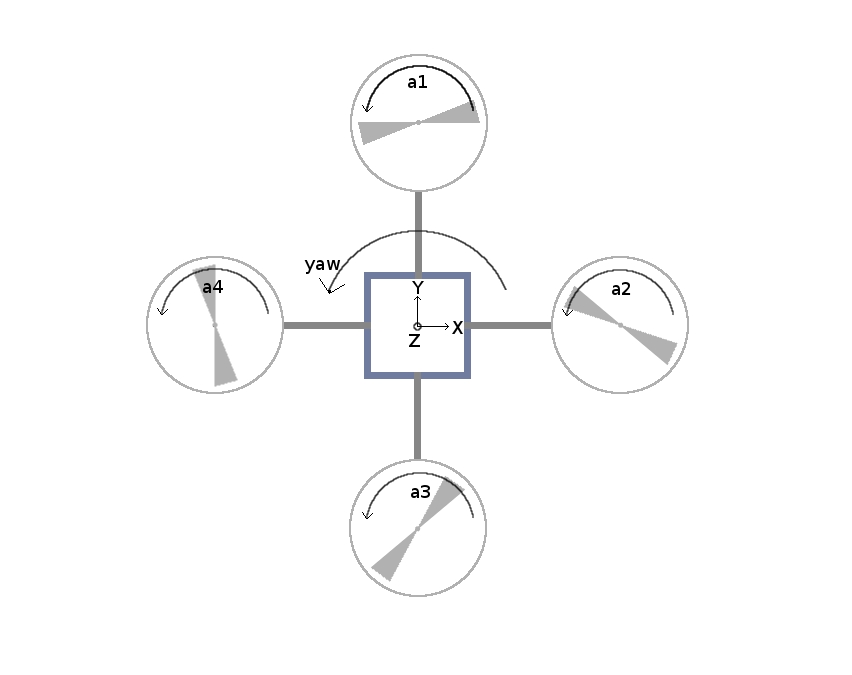
\includegraphics[width=0.75\textwidth]{quadrotor_states_actions.png}
    \caption{Quad-rotor schematic with states and actions depicted. All states and actions are continuous.}
\end{figure}

\section{Payload control for UAVs}

There has been some work to control the payload of an UAV directly using Control Theory \cite{PayloadControlTheory,PayloadControlTheory2}. These approaches again require a lot of knowledge about the system, including the tension in the joint. Some even approximate the system to be linear to be able to solve the resulting differential equations.

There has also been some work in controlling payloads of UAVs using Reinforcement Learning \cite{PayloadLSPI}. In this, Least Square Policy Iteration (LSPI) is used. Three different LSPI are used to track the x, y, and z dimensions. This has the disadvantage of these three learning policy iterations that can clash with each other. In the case of a quad-rotor, where the system is under actuated, the x and y dimensions are correlated.

\begin{figure}[H]
  \centering
    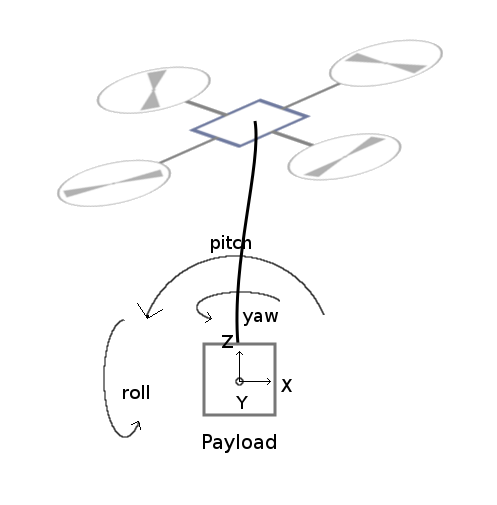
\includegraphics[width=0.5\textwidth]{payload.png}
    \caption{Quad-rotor with a payload attached using a non rigid body. States (cartesian co-ordinates and euler angles) of the payload are shown.}
\end{figure}

\section{Apprenticeship Learning}

In reinforcement learning a reward function is used which describes the task and the target that needs to be achieved. Reinforcement learning can be applied to tasks as ill defined as "drive the car well". This is not clear and has many many inherent meanings like "drive to the destination quickly", "do not crash into anything", "stop at red signals" and even more subtle meanings like "change lanes as little as possible", "move in smooth trajectories" and so on. In such cases, which are not clearly defined it is even more difficult to quantify the expected task and create a reward function.

Inverse Reinforcement Learning (IRL) is a field of Reinforcement learning where no reward function is given. Here, the agent tries to identify the reward function, given some pre-prepared behaviour of another agent. The pre-prepared agent is assumed to be an expert. This usually requires multiple demonstrations as the reward function is analyzed using these trajectories and policies.

Apprenticeship learning \cite{ApprenticeshipLearning} helps to solve this issue by learning a task from a mentor which already knows the target and is thought to be maximizing a reward function. The mentor is asked to perform the task and the trajectories and actions used by the mentor is stored in the memory of the agent. Then the agent uses this memory to help itself find a suitable policy for the task. A naive policy can be derived by identifying which transitions occur frequently in the mentors trajectories and which ones do not. The frequent transitions should give a larger reward while the transitions that do not occur give no or negative rewards. The mentor can even specify which trajectories are bad and should not occur for a more balanced reward function.

In the case of the continuous rewards and states like ours, it is impossible to count transitions and so the above method is not possible. A more structured approach to the analysis is required. In such cases the trajectories need to be time normalized and then stitched to find the optimal policy for the task.

\section{Predator Prey methods}

Predator Prey environments are dynamic systems where there are a few Predators and a few prey. The predators attempt to catch the prey while the latter attempts to escape. There are a few escape states where the predator is incapable of reaching, but the prey is - making those the end states. This work involves learning a second layer (high level control of the quad-rotor) to chase after a trajectory.

The Predator Prey systems are motivated from population theory \cite{PredatorPreyCoEvolution} where the population of animals is modelled. In such cases, there is food for prey (plants) planted at various points. These are considered to be static, but they can grow over time. The prey moves around eating or resting. Eating and resting allows them to conserve energy which is then used to escape from predators or find more food. If a prey or predator does not eat for too long, they may die. Population theory is used to spawn new predators and prey based on known distributions.

In a large number of cases, the Prey is considered a passive agent which simply moves in predefined paths like towards food and to a resting area (their home), or even simply a random motion. There has been a large amount of work to make the predator learn to catch the prey as quickly as possible. Most techniques \cite{PredatorPrey} keep a value function and use Temporal Difference (TD) algorithms to find this value function. This can also be done by a policy search method like PEGASUS.

Predator Prey environments typically focus on systems where the prey is a learning agent. Hence, the path taken by prey is not known a priori. This can be used on top of the quad-rotor control for actions like catching objects, finding other quad-rotors, etc. Also, the main concept in these tecniques is to catch the prey as soon as it can or catch it before the time ends. Hence, the policy learnt makes the predator move in the time optimal trajectory to catch the moving target.

%%%%%%%%%%%%%%%%%%%%%%%%%%%%%%%%%%%%%%%%%%%%%%%%%%

\chapter{PEGASUS}

PEGASUS \cite{PEGASUS} (Policy Evaluation-of-Goodness And Search Using Scenarios) is a technique devised by Andrew N. G. and Michael Jordan which finds a policy by searching through the whole policy space. It eliminates policies based on the "goodness" of it. Using the goodness quantification, it then attempts to find the next policy to check.

\section{Value of the policy}

In Reinforcement Learning there is already a notion of a policy as well as a value function. Here, the value of the policy or the "goodness" of the policy is defined as the value of the initial state ($s_{0}$) in an episode. This can also be thought of the total return the policy is capable of getting. Extending it to multiple episodes, the expectation over the distribution of initial states $\mathbb{D}$ is used:
\begin{equation}
  V(\pi) = \mathbf{E}_{s_{0} \sim \mathbb{D}} [ V^{\pi} (s_{0})]
\end{equation}

As the value of the policy is not known before hand, it needs to be estimated. To compute the value of the policy, the rewards for an episode need to be found and the return can then be found by discounting them based on time. The initial state ($s_0$) can be stochastic and is sampled from the distribution of initial states ($\mathbb{D}$). To get a better estimate, the value is averaged over multiple episodes. Consider a sequence of states ${s_{0}^{i}, s_{1}^{i}, s_{2}^{i}, ...}$ for the $i^{th}$ episode and $m$ episodes are run (to reduce the variance in the value of the policy). This can be written as:
\begin{equation}
  V(\pi) \approx \hat{V}(\pi) = \frac{1}{m} \sum_{i=1}^{m} V^{\pi} (s_{0}^{i})
\end{equation}

\section{Obtaining the optimal policy}

Now that a quantitative scalar has been found for the value of the policy, they can be compared. This comparison of the value is equivalent to coparing the policies itself. For example, A policy $\pi_{1}$ is considered better than another policy $\pi_{2}$ if $V(\pi_{1}) > V(\pi_{2})$. Hence, the optimal policy can be defines as:
\begin{equation}
  \pi^{*} = {\arg \max}_{\pi \forall \mathbf{\Pi}} {V(\pi)}
\end{equation}

In a problem where the actions are discrete and an episode terminates after $H$ steps, a policy is simply a sequence of $H$ actions from the action space. As the actions space is discrete, there will be a discrete set of policies. To be specific, there will be $|\mathbb{A}|^{H}$ policies at maximum. Here, if the value of the policies are found, by comparison, the optimal policy would be the one which has the maximum value.

However, in a problem where the actions are continuous it is not feasible to find the values of all the policies. In such a case, function approximation is used with a set of parametric functions for the policy. This parametric function can be anything, as long as it is continuous and can be defined by finite parameters ($\mu$). Wit this, the value of the policy can be written as:
\begin{equation}
  V(\pi) = V(\pi_{\mu})
\end{equation}

Hence, the value now becomes a function of a finite set of continuous variables $\mu$. This can be visualized as a $|\mu|+1$ dimensional graph which maps $\mu$ to $V$. In this multi-dimensional graph, the maximum value of the function needs to be found using a maximization technique. For example, gradient descent, stochastic gradient descent, BFGS algorithm, random search, etc. Using these techniques the maximum $V$ and hence the optimal policy $\pi^{*}$ can be found.

\begin{figure}[H]
  \centering
    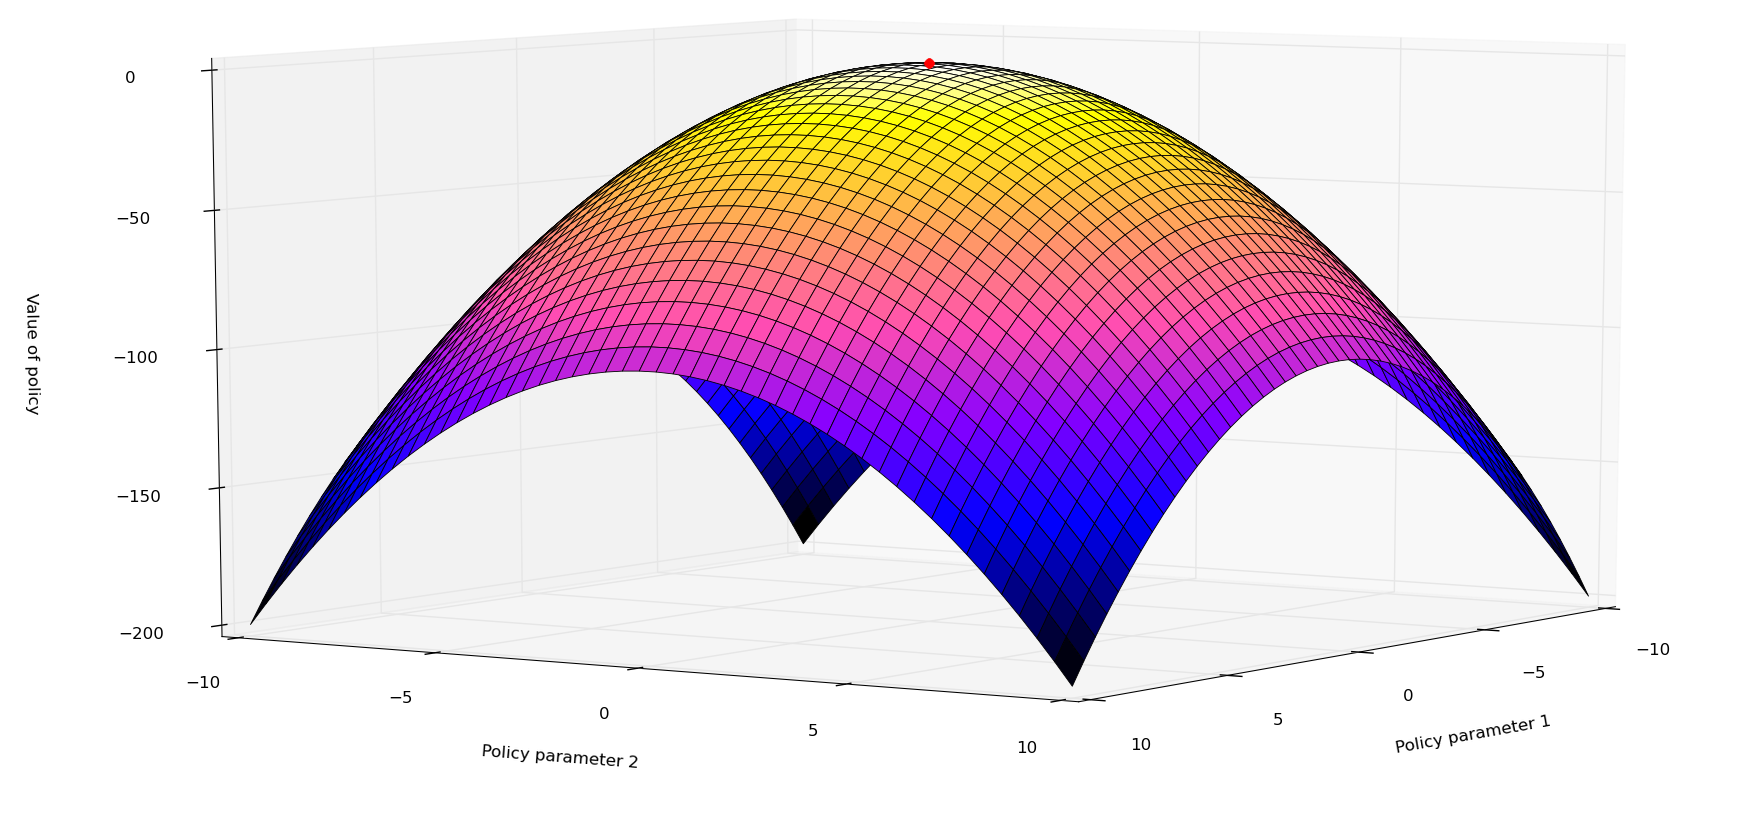
\includegraphics[width=\textwidth]{gradient_descent.png}
    \caption{An example of a policy with 2 parameters. The value of the policy at these parameters has been plot. The optimal policy is marked at the maximum value.}
\end{figure}

\section{Conversion of Stochastic MDP to non-stochastic POMDP}

The PEGASUS algorithm works for both MDPs and POMDPs. But, it involves running a specific scenario multiple times - and assumes the same transition function for the environment. If the transition function is not same, the value of the policy will have a large variance. Hence, it does not work well with stochastic transition functions.

This can be tackled by simply converting stochastic MDPs or POMDPs into an appropriate POMDP with a random seed that is not observed. Hence a new POMDP is created wihch has the state space of the states from the original MDP along with the random variables that will be used by the transition function. This potentially makes the new POMDP's state space infinite dimensional.

Let us take the original stochastic (PO)MDP as $MDP_{1}$ which has the state space $\mathbb{S}$. Now, an infinite set of random numbers generated from a true uniform random generator $[0,1]^{\infty}$ is sampled. A new POMDP $MDP_{2}$ which has the state space $\mathbb{S} \times [0,1]^{\infty}$ is created. This new POMDP $MDP_{2}$ has a environment that uses these uniformly random variables in it's state for any non-stochastic calculations it has. It is trivial to convert a uniform random variable into any other distribution like Bernouilli, Binomial or others as required. Hence, the transition function in $MDP_{2}$ is deterministic based on it's state space.

For implementation purposes, it is impossible to use state spaces with infinite dimensions, and this is not really needed. The episodes are truncated after $H$ steps, so only $H$ random variables would be used within these $H$ steps. This reduces the state space size to $\mathbb{S} \times [0,1]^{|H|}$. To reduce the memory complexity furthermore, only a seed needs to be added to the state space. This seed can initiate an appropriate random number generator for an episode.

\section{Application to helicopters}

PEGASUS has already been used in helicopters \cite{HelicopterPegasus}  by Andrew Ng, Jin Kim, Michael Jordan and Shankar Sastry. In their paper they describe using PEGASUS on a model they created of the helicopter which was used to learn. After the learning on this model, they implemented the policy learnt on the actual helicopter and obtained successful results.

There, they created the Model of the helicopter by getting trajectories from a human pilot. This is not an ideal method as the human pilot is incapable of using the helicopter in certain states and the transition function would be biased to better scenarios rather than worse ones. This introduces a bit of the model of the helicopter into the model inherently.

Next, they design a shallow neural network to make the policy class $\Pi$ that PEGASUS requires. The weights of the neural network are taken as the parameters of the policy that are learnt by PEGASUS. This neural network is specific for the helicopter and cannot be generalized to other UAVs with different dynamics.

The reward function used in this paper is the L2 norm of the difference between the expected position and the original position. It includes the x, y, z position as well as the yaw. And the linear velocities are included in this too, with the target velocity being 0. As this is specifically for hovering, they also have a negative reward for large actions, as jerky behaviour is not wanted. With this system, they were able to make the quad-rotor hover and move in lines successfully.

\begin{figure}[H]
  \centering
    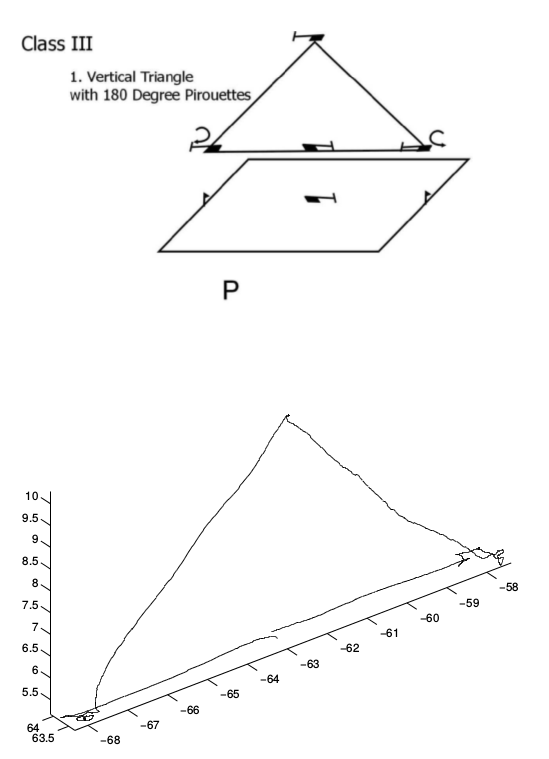
\includegraphics[width=0.4\textwidth]{pegasus_helicopter.png}
    \caption{Control of a helicopter using PEGASUS by Andrew Ng, Jin Kim, Michael Jordan and Shankar Sastry \cite{HelicopterPegasus}. A comparison of maneuver diagrams from RC helicopter competition\protect\footnotemark \space compared with actual trajectories from the model learnt by PEGASUS.}
\end{figure}
\footnotetext{Maneuver diagrams taken from http://www.modelaircraft.org}

\subsection{Aerobatics}

There has also been some later work on using PEGASUS along with Apprenticeship learning in helicopters to do complex tasks like aerobatics \cite{ApprenticeshipHelicopterAerobatics}. Apprenticeship learning provides an efficient method to create a reward function, and PEGASUS learns the policy based on the generated reward function.

To complement this, there has also been work on using PEGASUS for outright unstable states that are difficult for most human pilots. The work by Andrew Ng, Jin Kim, Michael Jordan and Shankar Sastry on Inverted helicopter flight \cite{InvertedHelicopterFlight} uses PEGASUS with an underlying controller. The underlying controller provides a flexibility to the system and generalizes it further.

\begin{figure}[H]
  \centering
    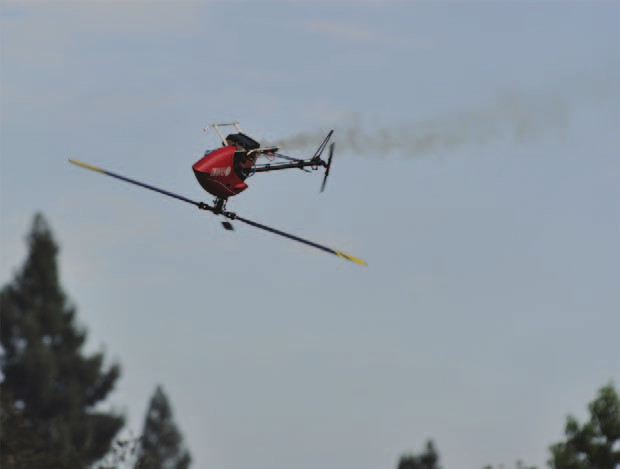
\includegraphics[width=0.5\textwidth]{pegasus_inverted_helicopter.png}
    \caption{Control of a helicopter to hover inverted using Apprenticeship Learning and PEGASUS by Andrew Ng, Jin Kim, Michael Jordan and Shankar Sastry \cite{InvertedHelicopterFlight}.}
\end{figure}

%%%%%%%%%%%%%%%%%%%%%%%%%%%%%%%%%%%%%%%%%%%%%%%%%%

\chapter{Simulation}

As stressed earlier, a simulated environment is the most important to implement PEGASUS. To emulate the quad-rotor, ROS \cite{ROS} is used - the well known open source Robot Operating System along with the physics simulator Gazebo \cite{Gazebo}.

\section{ROS and Gazebo}

ROS and gazebo provide a good API to modify parameters of a simulation, and are intended to provide a software layer on top of hardware. Hence, it is easy to replace the hardware with a simulated hardware. Along with this, it is possible to provide an interface to make controllers with easily configurable time steps and so on.

ROS also provides a method to isolate pieces of code from one another (called nodes) which fits well with the Reinforcement Learning framework where an Agent and Environment need to be isolated. Nodes can then communicate with each other using services or topics.

Topics are intended for continuous stream-like communication at specific intervals. Hence interrupts and streams are easy to create using topics. Topics provide only one way communication. Services provide a method to have 2 way communication. This is similar to calling a function from another node with specific arguments.

Gazebo provides a multi-robot simulation environment. It wraps the ODE and bullet physics engines and provides kinematic and dynamic simulation also. Gazebo is capable of simulating gravity, contact forces, joints and frictions but ignores aerodynamics and propulsion systems which are important factors to consider for a quad-rotor. Gazebo is slow with fluid systems and hence simulating air flow is complicated.

Hence, ROS and Gazebo do provide a good method of simulating

\section{Hector Quadrotor}

Hector Quad-rotor \cite{HectorQuadrotor} is a ROS package which helps to simulate quad-rotors in ROS and Gazebo. It is provided by Team Hector for Urban Search and Rescue (USAR) applications. Hector Quad-rotor was created specifically to path the issues that Gazebo has with simulating UAVs. It gives an easy method to import a quad-rotor model using the COLLADA format (exportable by Blender) while the collision model is modeled as a .stl mesh.

The propellers are modelled as discs as a trade-off between visual accuracy, collision detection and dynamics modeling. Modelling it as fans proved troublesome due to the collision detection which gave varied results with different physics time steps.

\begin{figure}[H]
  \centering
    \begin{subfigure}[c]{0.45\textwidth}
      \centering
        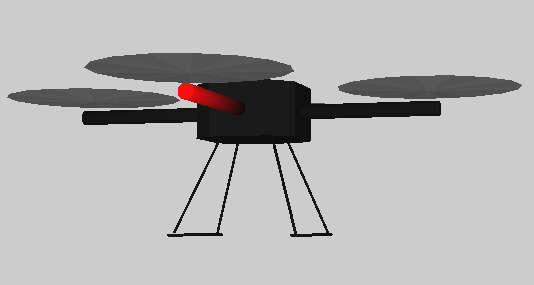
\includegraphics[width=\textwidth]{quadrotor_sim.png}
    \end{subfigure}
    \begin{subfigure}[c]{0.45\textwidth}
      \centering
        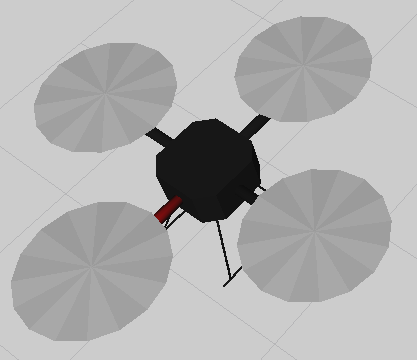
\includegraphics[width=\textwidth]{quadrotor_sim2.png}
    \end{subfigure}
    \caption{Quad-rotor simulated by Hector Quadrotor using ROS and gazebo.}
\end{figure}

The dynamics of the quad-rotor are based on Samir Bouabdallah's work \cite{QuadrotorDynamics}. It includes the flight dynamics, motor dynamics, and thrust calculations required for the system. Sensors have also been emulated using an error model like the Gauss Markov error model. Common sensors like IMU, barometric, ultrasonic, GPS and compass have been implemented in the package.

Hector Quad-rotor also provides a basic controller. The controller is implemented by separate cascaded PID controllers controlling roll and pitch movement, yaw rate and linear z velocity. This assumes that each axis and the altitude can be controlled independently. This is a valid assumption for quad-rotors for moderate deviations from the hovering state.

This controller is abstracted and has implementations to use any sort of input. The types of inputs that are possible are torque (wrench), position (pose), velocity (twist), and also motor velocity. This allows us to easily implement our own controller.

\section{Reinforcement Learning framework}

RL-Glue \cite{RLGlue} is a well known Reinforcement Learning framework which helps to write Agents and Environments that are independent of each other. RL-Glue works by using sockets which is very similar to how ROS nodes are implemented. RL-Glue has a thin wrapper for ROS called ROS-Glue, but this has become unsupported and is old.

Hester T. and Stone P. made a ROS package for their paper on TEXPLORE \cite{Texplore}. The rl-texplore-ros-pkg\footnote{https://github.com/toddhester/rl-texplore-ros-pkg} provides topics and messages which help in communicating between an agent and an environment. It can also handle multiple agents and has some popular algorithms already implemented.

This package however did not integrate gazebo into the environment, and our own reinforcement learning package\footnote{https://github.com/AbdealiJK/quadrotor\_control} was created, which is integrated with hector\_quadrotor and gazebo. The texplore package also did not implement Pegasus. This modified package is able to communicate with gazebo as part of the environment and can use the models of the gazebo simulator and converts it into a state. It also has the ability to run gazebo in finite time steps, pausing the simulator between them.

\subsection*{Agent}

The agent is a ROS node which implements from the abstract class provided in the texplore package \texttt{Agent}. It implements the functions first action, last action and next action which are intended to initiate the episode, end the episode and continue to the next time step of the episode respectively.

The Agent automatically transmits the action using the RLAction message on the topic \texttt{rl\_agent/rl\_action}. The message is an array of any length of float32 type. Hence, it is possible to supply any number of actions for a complex agent.

\subsection*{Environment}

The environment is a ROS node which implements from the abstract class provided in texplore package \texttt{Environment}. It implements the function sensation, apply, terminal, and reset. The function sensation is the state or the observation from the environment that the agent is capable of observing. The function apply takes in the action given by an agent and applies that to the environment. The terminal and reset functions act as destructors and constructors to reuse the environment in various episodes.

The environment transmits the state information using the RLEnv message on the topic \texttt{rl\_env/rl\_state\_reward}. The message has 3 variables. An array of any length which has float32 items which is the state or the observable state by the agent. A scalar of type float32 which is the reward obtained by the last step (In the start state, this is ignored). And finally a boolean which indicates whether the state is a terminal state or not.

An environment named Hector Quad-rotor has been implemented which passes the action from the agent to the gazebo environment as a twist state. The sensation function is also implemented in such a way as to wait for gazebo to complete a transition step and return back the observable state from this. For all this a random seed can be set in gazebo to create the repeatable scenarios required by PEGASUS.

%%%%%%%%%%%%%%%%%%%%%%%%%%%%%%%%%%%%%%%%%%%%%%%%%%
\chapter{Quad-rotor Dynamics model}

\section{States and Input}
Quad-rotor dynamics can be controlled with the rotor thrusts. This is used to change the altitude, pitch, roll, and yaw of the quad-rotor. The effect the rotor thrust has on the roll, pitch, yaw, and altitude can be found using the model of the quad-rotor.

Combining the revolutions per minute (rpm) of the 4 rotors makes it possible for the quad-rotor to turn, and move in various ways. The following configurations are possible:

\begin{figure}[H]
  \centering
    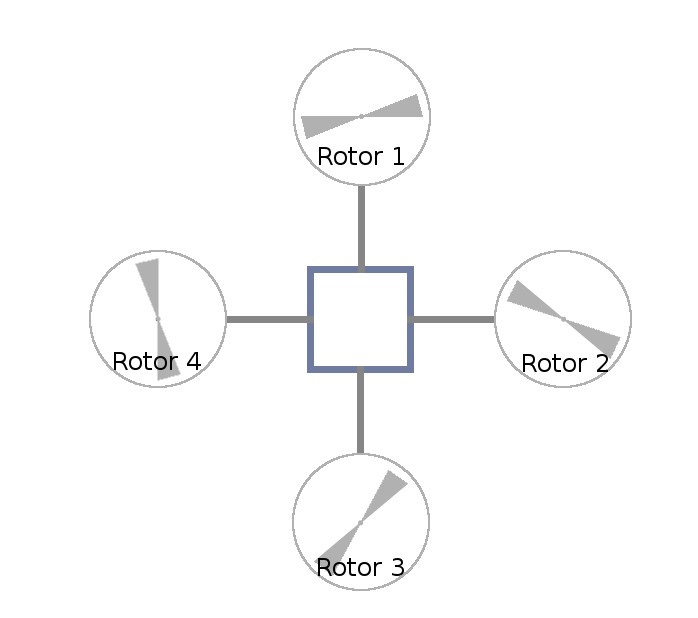
\includegraphics[width=0.5\textwidth]{quadrotor_rotors_names.png}
    \caption{The four rotors of the quad-rotor which are used in different configurations for motion.}
\end{figure}

{\bf Altitude (z)}: To change altitude (in the positive z direction) equal thrust is applied to all the rotors. Alternate rotors are given thrust in opposite directions so that the torque does not cause the quad-rotor to change it's pitch and roll. For example, if Rotors 1 and 3 are moving in the clockwise direction Rotors 2 and 4 need to move in anti-clockwise direction. This is also required for hovering as there is a constant gravitational force acting downward which needs to be countered.

\begin{figure}[H]
  \centering
    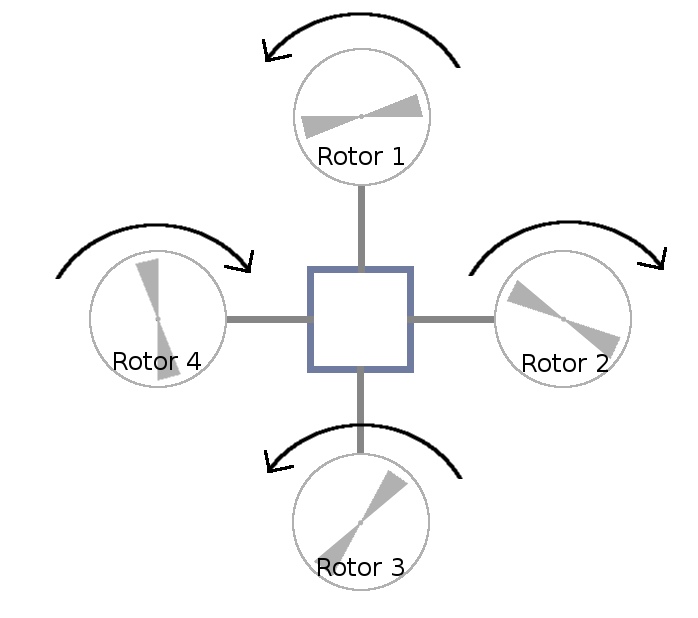
\includegraphics[width=0.5\textwidth]{quadrotor_rotors_altitude.png}
    \caption{The configuration of the 4 rotors of a quad-rotor to change altitude.}
\end{figure}

{\bf Yaw}: To change the yaw while hovering, the thrust applied to the rotors need to be different so that torque is not zero. But as no force force in the z direction is wanted, alternate rotors have the same thrust. For example, Rotors 1 and 3 need the same thrust and Rotors 2 and 4 also need the same thrust. But one pair will have a lesser thrust than the other depending on the direction in which yaw needs to be changed.

\begin{figure}[H]
  \centering
    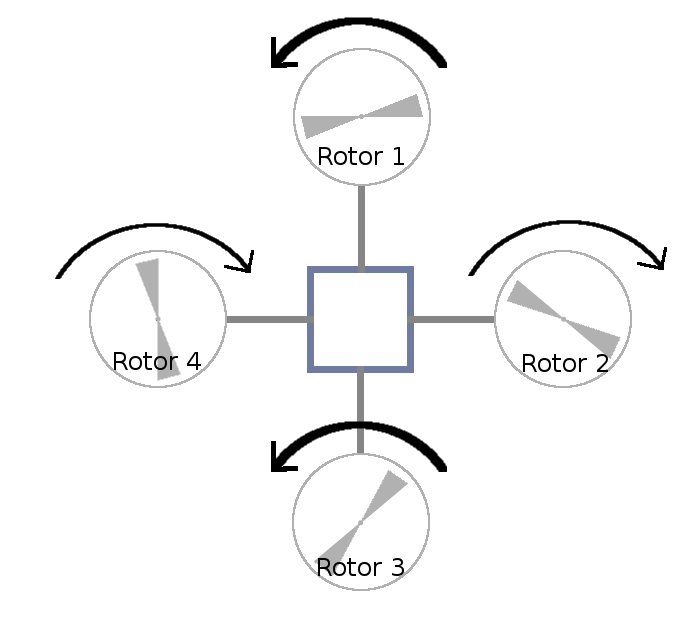
\includegraphics[width=0.5\textwidth]{quadrotor_rotors_yaw.png}
    \caption{The configuration of the 4 rotors of a quad-rotor to change yaw.}
\end{figure}

{\bf Pitch and Roll}: In a quad-rotor, it can be observed that the x and y directions (or the pitch and roll angles) are symmetric. This symmetric nature let's us use the similar control logic for both these directions. To change the pitch and roll, the alternate motors move in opposite directions to counter torque appropriately. Here, one pair of diametrically opposite motors have the same thrust while the other pair does not. This causes the quad-rotor to turn toward the direction of the lesser rotor. For example, if Rotors 2 and 4 have the same thrust, Rotor 1 would have more thrust than Rotor 3 (or vice-versa). Similarly, if Rotors 1 and 3 have the same thrust the quad-rotor would move in the other symmetric direction.

\begin{figure}[H]
  \centering
    \begin{subfigure}[c]{0.45\textwidth}
      \centering
        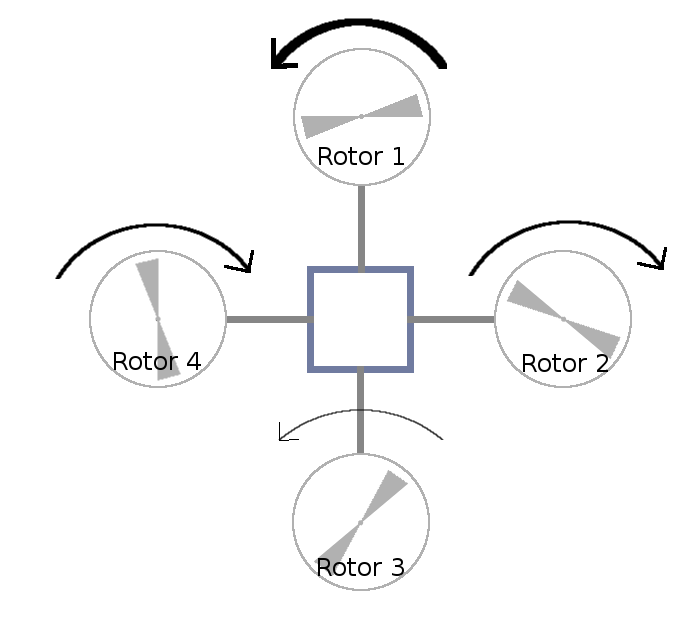
\includegraphics[width=\textwidth]{quadrotor_rotors_roll.png}
        \caption{}
    \end{subfigure}
    \begin{subfigure}[c]{0.45\textwidth}
      \centering
        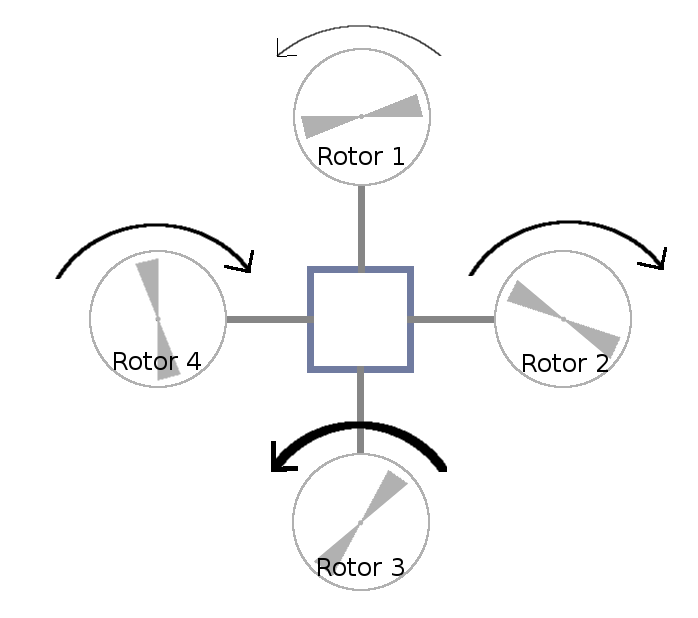
\includegraphics[width=\textwidth]{quadrotor_rotors_pitch.png}
        \caption{}
    \end{subfigure}
    \caption{The configuration of the 4 rotors of a quad-rotor to change roll and pitch.}
\end{figure}

\section{Model structure}

The quad-rotor dynamics have been documented by Samir Boubdallah and Roland Siegwart for the OS4 project \cite{QuadrotorDynamics}. This is the same modelling that is used in the Hector Quad-rotor package.

In the paper, each part of the quad-rotor is modelled, starting from the motors. The motor is taken to be a simple DC motor where the thrust $T$ is proportional to the vertical force acting on all the blade elements. The horizontal force (called Hub Force $H$ is found by calculating the resultant horizontal force and the drag $Q$. is found using a similar method.

Once the basic linear forces have been accounter for, the angular forces are found. The angular forces include the Rolling moments, Pitching moments, and Yawing moments. They go on to find the dynamic equation of the BLDC rotors also, as this would contribute to the moments to a small extent. This is found using a simple first order transfer function - to recreate the dynamics the propeller would acheive between the set-point required and the actual speed.

Using these individual forces, the net force on the quad-rotor can be calculated. This gives a set of equations defining the moments and forces (See equation 7 in Samir Boubdallah and Roland Siegwart's work \cite{QuadrotorDynamics}). Using this, it is now possible to define the the transition function as:

\begin{equation} \begin{split}
  f(\bar{S}, \bar{U}) = \left\{
    \begin{array}{c}
      \dot{\phi} \\
      \dot{\theta} \dot{\psi} a_{1} + \dot{\theta} a_{2} \omega_{r} + b_{1} U_{2} \\
      \dot{\theta} \\
      \dot{\phi} \dot{\psi} a_{1} + \dot{\phi} a_{4} \omega_{r} + b_{2} U_{3} \\
      \dot{\psi} \\
      \dot{\theta} \dot{\phi} a_{5} + b_{3} U_{4} \\
      \dot{z} \\
      g  - (\cos{\phi} \cos{\theta})\frac{U_{1}}{m} \\
      \dot{x} \\
      u_{x} \frac{U_{1}}{m} \\
      \dot{y} \\
      u_{y} \frac{U_{1}}{m}
    \end{array}
  \right\}
\end{split} \end{equation}

Where $\bar{U}$ is the action which is a 4 dimensional vector (1 action per rotor). The constants $m$, $a_{i}$, and $b_{i}$ are system parameters that can be calculated from properties like moment of inertia, mass, etc. $u_{j}$ is the projection from Spherical co-ordinates to Cartesian of a unit vector in the $j$ dimension in Cartesian co-ordinates.

This model is useful, as it helps to formulate the best policy class that can be used for this system in the case of PEGASUS.

%%%%%%%%%%%%%%%%%%%%%%%%%%%%%%%%%%%%%%%%%%%%%%%%%%%%%%%%%%%%
\chapter{Apprenticeship Learning}

Apprenticeship learning or Apprenticeship via inverse reinforcement learning \cite{ApprenticeshipLearning} is a concept that helps to perform complex trajectories that are not necessarily stable. These unstable trajectories are difficult to learn using the traditional reinforcement learning as the reward function is not easy to define.

Consider the case of the quad-rotor performing aerobatic stunts. In specific, take the case of the quad-rotor performing a flip. It is easy to describe the target trajectory as a flip, but it is difficult to create a closed form reward function for the same.

The approach followed in the case of the quad-rotor is as follows:

\begin{itemize}
\item{{\bf Build a baseline model}

Collect some flight data by flying the quad-rotor in various ways. Use this to estimate the parameter variables for the model defined in Samir Bouabdallah's work \cite{QuadrotorDynamics}. To reduce the error in estimating the model use a large number of maneuvers and as many states as possible.}

\item{{\bf Estimating the intended trajectory}

Now, the mentor that the apprenticeship will learn from performs a few flips. The state and action information is recorded during the flips. Now, as the mentor is human, the demonstrated trajectories will not be as accurate as possible. Some noice is assumed in all the demonstrated trajectories but the demonstrated trajectories together can be used to put together a intended trajectory. This is the main crux of the apprenticeship learning framework.}

\item{{\bf Control}

Once this intended trajectory is identified, a reward function is chosed that penalizes the agent if it deviated from the trajectory. This is required as the intended trajectory may not be possible for the quad-rotor to perform.}

\end{itemize}

In the above steps, apprenticeship learning contributes in the second step - where the trajectory is estimated using the demonstrated trajectories. Creating a model is an estimation problem \cite{EstTheo} which can be done easily and is based on the model. Controlling the quad-rotor using the estimated intended trajectory can be done using pure control theory methods like PID or can use methods like RL control and PEGASUS.

A hand engineered trajectory is difficult to form in complex cases. The apprenticeship learning setting relies on the expert rather than a hand-engineered trajectory. In this section, a method of inferring the expert's intended trajectory from a set of demonstrations is provided.

$M$ different demonstrated trajectories are given with time steps $N^k$ for $k = 0, 1, 2, ..., M-1$. Each trajectory can be defined as a set of states (position and orientation) and inputs (motor velocities) which are concatenated into a single vector $\mathbf{y}$:
\begin{equation}
  y_{t}^{k} \quad \text{for} \; t = 0, 1, 2, ..., N^{k}-1 \text{ and } k = 0, 1, 2, ..., M-1
\end{equation}
And our aim is to find the intended "hidden" trajectory denoted as:
\begin{equation}
  x_{t}^{k} \quad \text{for} \; t = 0, 1, 2, ..., T-1
\end{equation}

One issue here is that the time steps of each demonstrated trajectory is different, and there needs to be some way of identifying which time period of the trajectory in one demonstrated trajectory is related to a particular time period in the other. Hence some notion of time synchronization needs to be used and implemented.

Another issue is that of using the state and action to identify the intended state at every time step. This can be treated as a scenario where multiple sensors are observing the agent and there is some inherent noise in the observation. This sensor fusion and smoothening of time series can be performed by the well known Kalman Filter.

\section{Generative Model}

A generative model is a model that generates observable states given some hidden model parameters. The generative model in this context tries to create the transition function - if the state and action of the agent are known, the state at the next time step is predicted. This generative model is needed to make a Kalman filter to smoothen the trajectories.

The dynamics model has already been created by Samir Bouabdallah \cite{QuadrotorDynamics} and the intended trajectory will have the constraint:
\begin{equation}
  x_{t+1} = f_{t} (x_{t}) + {\omega}_{t}^{(x)}, \qquad \omega_t^{(x)} \sim \mathcal{N} (0, \Sigma^{(x)})
\end{equation}

Each demonstrated trajectory maps to the intended hidden trajectory with some noise. Hence, there are some hidden variables present in the system that can be computed based on the observed demonstrations from the expert. This can be written as:
\begin{equation}
  y_{t}^{k} = h(x_{\tau_t^k}) + {\omega}_{t}^{(y)}, \qquad \omega_t^{(y)} \sim \mathcal{N} (0, \Sigma^{(y)})
\end{equation}

Where, $\tau_t^k$ is the time step in the intended trajectory mapped to the observed trajectory at time step $t$. These time indices $\tau_t^k$ are not known and need to be found. There is no error at the start of the demonstration, and so $\tau_0^k = 0 \forall k$. A reasonable approximation of the total time steps in the hidden trajectory is twice the average of the demonstrations:
\begin{equation}
  T = 2 \left( \frac{1}{M} \sum_{k=1}^{M} N^k \right)
\end{equation}

\todo{Add image of the tau warping 2 trajectoryes (circles and arrows)}

In the generative model, there are other errors that creep in, and hence it needs to be extended. For example, it is often difficult for the expert to keep the quad-rotor centered about a fixed position. The demonstrated trajectory hence has demonstration drift which can be accounted for. This can be done using a gaussian noise model. There may be some prior knowledge about the states and actions in the trajectory which can also be added to the model. Incorporating all these errors, the final extended generative model can be seen in Section 4.1.3 of Pieter Abeel, Andrew Ng, and Adam Coates' work \cite{ApprenticeshipHelicopterAerobatics}.

\section{Trajectory Estimation}

The learning algorithm used in the original helicopter aerobatics paper \cite{ApprenticeshipHelicopterAerobatics} finds the time steps of the intended trajectory, the time index transition probabilities, as well as the error covariances by maximizing the joint likelihood of the observed trajectories $y^k$:
\begin{equation} \label{eq:ApprenticeshipJointProbability}
  \max_{\tau, \Sigma^{(\cdot)}, \mathbf{d}} \log \mathbb{P}(\mathbf{y}, \rho, \tau ; \Sigma^{(\cdot)}, \mathbf{d})
\end{equation}

Once the $\tau$, $\Sigma^{(\cdot)}$, and $\mathbf{d}$ are found, the intended trajectory $x$ can be found using these parameters and maximizing the joint likelihood of observing the demonstrated trajectories $y$.

The joint likelihood in Equation \ref{eq:ApprenticeshipJointProbability} is difficult to compute as $\tau$ is not known. This gives a large number of permutations to attempt. Hence, $\tau$ is set as a latent variable and Expectation Maximization is used to maximize this function. Then, to do the time mapping, dynamic time warping \cite{DTW} is used.

Hence the effective algorithm for apprenticeship learning has two steps:
\begin{itemize}
\item{{\bf Dynamic Time warping}: Use the currently estimated intended trajectory to find the time step mapping between the intended trajectory and the demonstrated trajectories.}
\item{{\bf Estimate the intended trajectory}: Use the mapped time states to estimate the intended trajectory using the EM algorithm applied to a non-linear dynamical system with Gaussian noise \cite{NonLinearEMKalman}.}
\end{itemize}

\subsection{Dynamic Time Warping}

Dynamic time warping \cite{DTW} has been used in multiple spheres. It is an algorithm that computes the similarity between two time series which may vary in time. Dynamic time warping has been applied to temporal sequences like video, audio, and graphics. It has been seen in  numerous speech recognition literature to cope with different speaking speeds.

What DTW does is that it finds the optimal match between the given sequences. It warps the time dimension non-linearly in the sequences to find the transform that makes the series the most similar based on a given metric. The alignment of the time dimension of two sequences is the feature that's needed to find the trajectories.

To visualize the DTW, often the time dimensions of the two series are plotted in a graph. In this graph, any one-to-one function (i.e. monotonously increasing function) will be a transformation in the time dimensions of the series. When two series which have the same speed are warped with DTW, the transformation will be plotted as the diagonal of the graph as the time dimensions do not need to be transformed at all.

Although the DTW can provide good results, often it provides the optimal result which intuoitively is wrong. Here, the concept of windowing is introduced, which constrains the mapped non-linear transformation of the time dimension to be "not too large". Windowing essentially constrains the DTW's warped time dimensions to be close to the diagonal in the visualized graph. This ensures that the warping isn't too severe.

One major concern is how to window the DTW. There have been many attempts to create smart methods of doing this. Some popular methods are itakura windowing, sakoechiba windowing, and slanted-band windowing. Each has it's own benefits and disadvantages and no single windowing technique is better than the rest.

\todo{Add pictures indicating the window types}

\subsection{EM with Kalman Filters for non-linear dynamical systems}

Kalman filters \cite{KalmanFilters} also known as Linear Quadratic Estimation (LQE) are another widely used concepts in time series. It is an algorithm that uses a series of measurements observed over time and produces estimates of a hidden variable which is more precise than estimating it from a single value.

One common use of Kalman filters is to get accurate information from sensors. It can handle sensors which temporarily stop working, and even filters out noise due to measurement or due to other physical factors. Kalman filters estimate the covariance and the mean of the hidden variable using observations.

A Kalman filter can be used for filtering, smoothening, and predicting.
\begin{itemize}
\item{{\bf Filtering} is the method of using the pervious data and current data to get a better estimate of the hidden variable ($\mu_{t|t}$).}
\item{{\bf Smoothening} is the method of using all the data available to get a better estimate of the hidden variable at a given time ($\mu_{t|T}$).}
\item{{\bf Filtering} is the method of using the pervious data to predict what the hidden variable at the next time instant will be ($\mu_{t|t-1}$).}
\end{itemize}

In scenarios where the model noise and the observation noise is not known can benefit from Kalman Filters along with Estimation Maximization. The EM based method has the E and M steps as normal EM implementations. The Expectation step smoothens the hidden time series and the Maximization step finds the covariance $Q$ and $R$ of the noise/uncertainity. This is done recursively until the estimated covariance of the noise converges.

Kalman filters are also commonly used to fuse data from multiple sensors to give an even more precise reading that each sensor individually. This is called sensor fusion \cite{KalmanFiltersFusion}. In our case, each trajectory is taken as a separate sensor and the data from these sensors are fused to obtain the intended hidden trajectory. This uses the data from multiple demonstrated trajectories  to obtain a better estimate than just one demonstration.

%%%%%%%%%%%%%%%%%%%%%%%%%%%%%%%%%%%%%%%%%%%%%%%%%%
\chapter{Position control}

As described earlier, velocity control has already been implemented in the Hector Quadrotor package. This is simply an abstraction from the motor to velocity of the quad-rotor itself. This is deterministic and is based on the model information of the quad-rotor. No learning takes place here.

On top of velocity, the next step is to establish a position control using PEGASUS. Here, when doing the learning, the quad-rotor learns to fly without a payload (by itself). Then the learnt policy is fine tuned for a particular payload. This benefit of this system is that the learning for the payload is much faster because the initial policy there is close to the optimal policy.

Hence, the payload's policy is abstracted out from the quad-rotor policy. This enables us to train a model to learn multiple different payloads faster. And the policy learnt from the quad-rotor can be easily transfered from one payload to the other easily.

\section{Quad-rotor control}

A typical implementation of PEGASUS in our case would have atleast 4 paramters in our policy class (for roll, pitch, yaw, and altitude) that need to be trained. Gradient descent is used to find the maximum valued policy in the PEGASUS algorithm.

The {\bf state} has 8 terms, of which 4 are independent (they can be calculated from the other 4). It captures the absolute position of the robot from a given origin. This can be found using external sensors like a set of cameras pointing a the quad-rotor or onboard sensors like IMU and altimeter. The state vector is:
\begin{equation}
  State = s = [x, y, z, \omega, \dot{x}, \dot{y}, \dot{z}, \dot{\omega}]
\end{equation}
Where, $(x, y, z)$ is the position of the center of mass of the quad-rotor at any given time, and $\omega$ is the yaw of the quad-rotor. The state could potentially also include the roll and pitch of the quad-rotor - but no significant improvement was found using those parameters. Theoretically the pitch and roll are correlated to the velocity $(\dot{x}, \dot{y}, \dot{z})$ and so offer no new data to the state.

For the origin, the relative position of the quad-rotor from the target position is used. This allows us to not be constrained in a specific area in space. This is bolstered by the intuitive observation that the policy wouldn't change based on absolute position, rather it would change based on the relative position of the target and the robot. This reduces learing time drastically and makes the polciy generalized over space.

The {\bf action} used in our implementation are the abstracted velocities after the velocity control. The action vector is:
\begin{equation}
  Action = a = [\dot{x}, \dot{y}, \dot{z}, \dot{\omega}]
\end{equation}
The action used is the abstract velocity, as this allows us to be flexible when choosing the system. This same PEGASUS formulation can be used if the robot is an octa-quad or similar UAVs, without any change in the position control. The benefit here, is that if a multi rotor UAV finds that there is a defect in one of it's motors, it is easy to switch over to another policy which does not use this motor. This enables the UAV to be smarter and control damage without affecting performance.

The {\bf policy} class used for the PEGASUS is from the above mentioned state space to the action space $\pi: S \rightarrow A$. The policy is written as:
\begin{equation}
  Policy = \pi(s) = \left\{
    \begin{array}{c}
      c_1 \times x + c_2 \times \dot{x} \\
      c_3 \times y + c_4 \times \dot{y} \\
      c_5 \times z + c_6 \times \dot{z} \\
      c_7 \times \omega + c_8 \times \dot{\omega} \\
    \end{array}
  \right\}
\end{equation}


The {\bf reward} used is the L1 norm of the deviation from the target. The reward is negative, and so the maximum reward that the quad-rotor can acheive is zero. A zero reward is got when it hovers exactly at the target. The reward function is written as:
\begin{equation}
  Reward = r(s) = - |x - x_0| - |y - y_0| - |z - z_0| - K \times |\omega - \omega_0|
\end{equation}

\begin{figure}[H]
  \centering
    \begin{subfigure}[t]{0.45\textwidth}
      \centering
        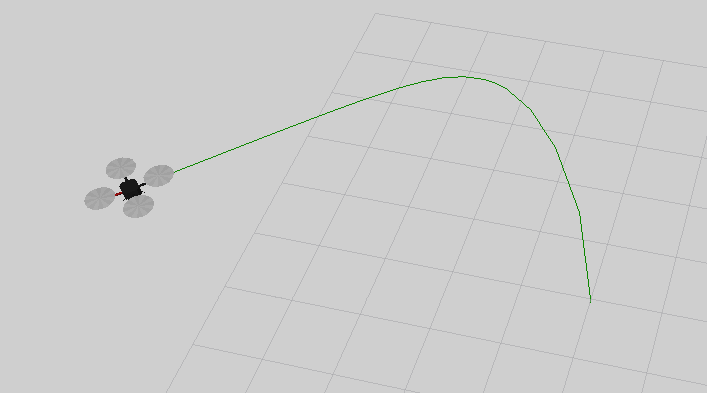
\includegraphics[width=\textwidth]{quadrotor_position_control.png}
    \end{subfigure}
    \begin{subfigure}[t]{0.45\textwidth}
      \centering
        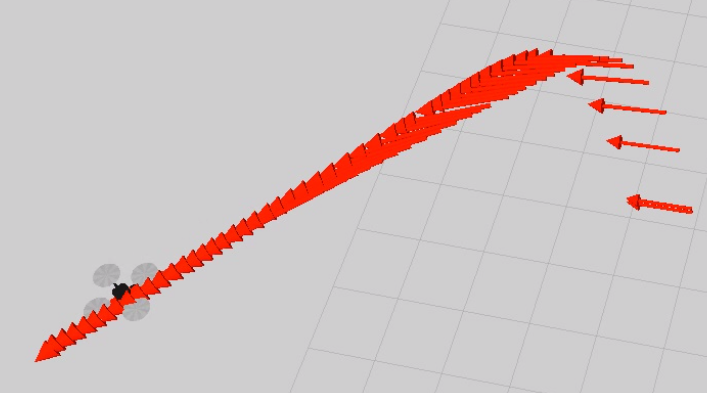
\includegraphics[width=\textwidth]{quadrotor_position_control2.png}
    \end{subfigure}
    \caption{Quad-rotor moving using the trained policy by PEGASUS to move from one position (x, y, z, $\protect\omega$) to another.}
\end{figure}

The roll and pitch are not considered in the target nor the state, as a quad-rotor cannot hover at a position with a non-zero roll and pitch. Hence, the target's roll and pitch is always assumed to be zero. It is impossible to learn a policy which allows the quad-rotor to maintain a specific roll and pitch as it would simply move to another orientation, and when returning back to the $(x, y, z, \omega)$ the roll and pitch will again change.

Trying to maintain a roll and pitch is the specific case of unstable targets. In aerobatics, veteran human pilots attempt to maintain the quad-rotor in an inverted state. Our method gives the quad-rotor a negative reward in such cases as this is a difficult method to learn. The policy is unable to handle a unstable like this, and things spiral out of control.

\begin{figure}[H]
  \centering
    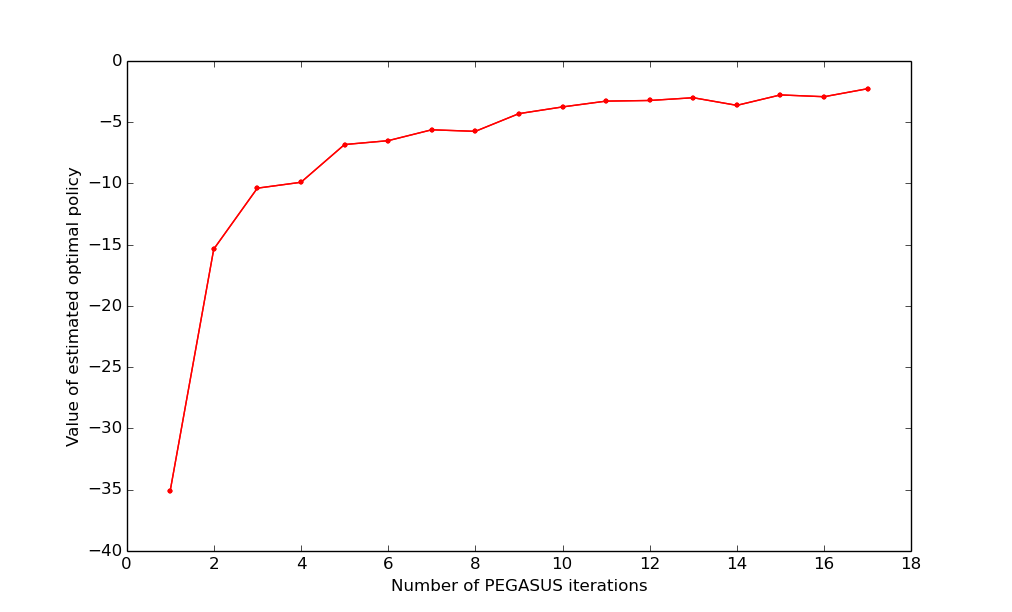
\includegraphics[width=\textwidth]{quadrotor_position_control_time.png}
    \caption{Value of best policy found with each iteration of PEGASUS to move to a given target position $(x, y, z, \omega) = (5, 5, 5, 60\protect^{\circ})$ with stochastic wind.}
\end{figure}

Unstable states like the ones seen in aerobatics have the problem that the mechanism is too complex to model into simple closed form reward functions. Apprenticeship learning is something that would make this possible, as was done by Andrew Ng, Jin Kim, Michael Jordan, and Shankar Sastry in their work with inverted helicopters \cite{InvertedHelicopterFlight}.

\subsection{Time analysis}

The gradient descent method attempts to move in small steps in various directions and approximates the gradient of this multi-dimensional function. Hence, if there are $P$ parameters in the policy class, it calcuates the value of the policy $2 \times P$ times. Now if gradient descent is run $T$ times, the number of episodes that are run are $2 \times H \times P \times T$ where $H$ is the number of times the value of the policy is averaged over in 1 scenario.

A few parameters are independent in the chosen policy class. For example, $c_1$ and $c_2$ can be learnt independent of $c_7$ and $c_8$. But, all the parameters depend on $c_5$ and $c_6$ as they need to be able to hover. Hence by learning this a few variables at a time, it increases the chance of converging faster. This basically means multiple policy gradients can be run on various parameters independently in the PEGASUS algorithm.

Currently, ODE does not have GPU capabilities and so is forced to run in the CPU. Because of the nature of physics simulations (where every time step depends on the last) it is not possible to parallelize the steps. Running gradient descent in smaller subsets of the policy also makes it possible to parallelize the learning over multiple computers, and hence faster.

\section{Payload control}

The next step is to control the payload's position. Here, a payload is suspended on the quad-rotor with some freedom at the joint. This makes the payload move in it's own path, not fixed by the quad-rotor's path. Hence, the inertia the payload accumulates cannot be directly controlled.

\begin{figure}[H]
  \centering
    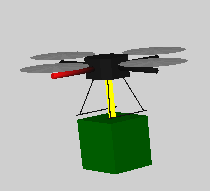
\includegraphics[width=0.4\textwidth]{payload_sim.png}
    \caption{Payload on quad-rotor simulated by Hector Quadrotor, ROS, and gazebo.}
\end{figure}

The state vector used in PEGASUS is again the same as above, but it uses the state of the payload rather than that of the quad-rotor. Also, the target state that needs to be acheived is the payload's state.

The action is still the action of the quad-rotor. There is no action that can be done directly on the payload as the joint is not actuated. Hence, the only variables that are controllable are the velocities (linear and angular) of the quad-rotor. It is interesting to note that when using the above reward and policy class the payload moves in a smooth trajectory without much deviation from the intended behaviour. This is without any state information of the quad-rotor. This is probably because the state information of the quad-rotor is highly correlated to the state of the payload. If more joints need to be added (like a chain for example), this would not hold true and a better policy would need to be considered.

With 3 chain links, although the policy class used was sub optimal, the value function of the payload's policy converged to a better policy than the original one without the payload (a policy with lower value). Hence, the policy was fine tuned to this payload. If the joint angles are known using an angular position sensor, the policy found can be made even more precise as the state representation will be better.

\begin{figure}[H]
  \centering
    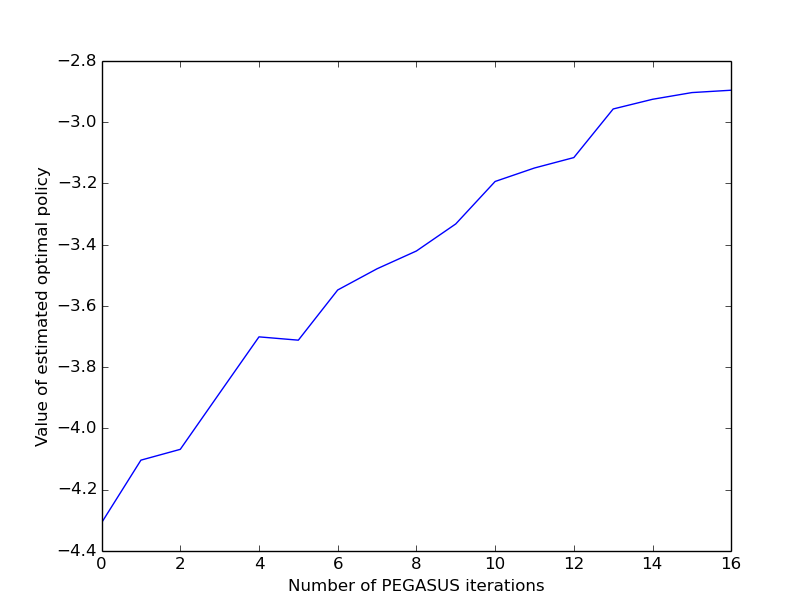
\includegraphics[width=0.8\textwidth]{payload_position_control_time.png}
    \caption{Value of best policy with each iteration of PEGASUS to move to a given target position $(x, y, z, \omega) = (5, 5, 5, 60\protect^{\circ})$. The payload is attached with a chain consisting 3 links and the initial policy is the optimal policy without the payload.}
\end{figure}

\begin{figure}[H]
  \centering
    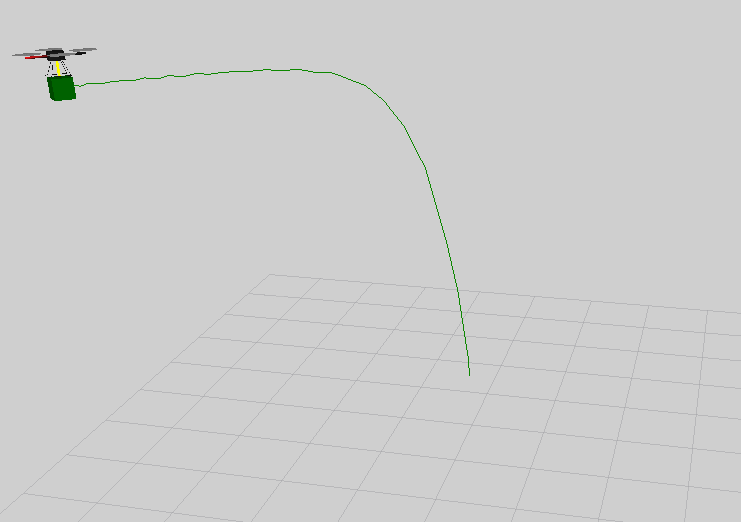
\includegraphics[width=0.6\textwidth]{payload_position_control.png}
    \caption{Payload moving using the trained policy by PEGASUS to move from one position (x, y, z, $\protect\omega$) to another.}
\end{figure}

%%%%%%%%%%%%%%%%%%%%%%%%%%%%%%%%%%%%%%%%%%%%%%%%%%
\chapter{Trajectory control}

Once the velocity and position control are established, the quad-rotor or payload need to be controlled to move in trajectories. A trajectory is a spatial function which relates position and time. Hence, the next step is to control the position that the quad-rotor or payload attains at a specific time, introducing the new dimension of time.

There are multiple different methods to trace a trajectory after position or velocity control are established. Each technique has it's strengths and weaknesses. These methods which use a planned trajectory are analyzed and compared. This trajectory information is then used to find the optimal controls to give to the quad-rotor to acheive the trajectory.

If the trajectory is not known, the predator prey models described above can be used. Also, for unstable trajectories, the PEGASUS control policy is not apt and so apprenticeship based methods are used.

\section{Checkpoints based trajectory control}

A checkpoint is defined as a set of points on the trajectory. The quad-rotor or payload is expected to go through these checkpoints in the appropriate order. Hence, this is anologous to the quad-rotor going through loops which are predefined in an arena. The checkpoints do not have specific timestamps here, but there is an ordering that needs to be followed.

The quad-rotor or payload is considered to have gone through a checkpoint if it moved "close" to that point. For example, consider a checkpoint that is defined by the position information:
\begin{equation}
  [x_c, y_c, z_y, \omega_c]
\end{equation}

The quad-rotor or payload is considered to have gone through this checkpoint if their position is within a spatial neighbourhood of the checkpoint. This can be written as:
\begin{equation} \begin{split}
  |x - x_c| &< \epsilon_x \\
  |y - y_c| &< \epsilon_y \\
  |z - z_c| &< \epsilon_z \\
  |\omega - \omega_c| &< \epsilon_\omega
\end{split} \end{equation}
The $\epsilon_i$ would be different for $\omega$ as compared to the others because of the units. Also, notice that $\epsilon_z$ need not be very small as altitude control of the quad-rotor is considerably better than control in x or y dimensions. Larger errors in altitude can be easily corrected when prusuing the next checkpoint.

\begin{figure}[H]
  \centering
    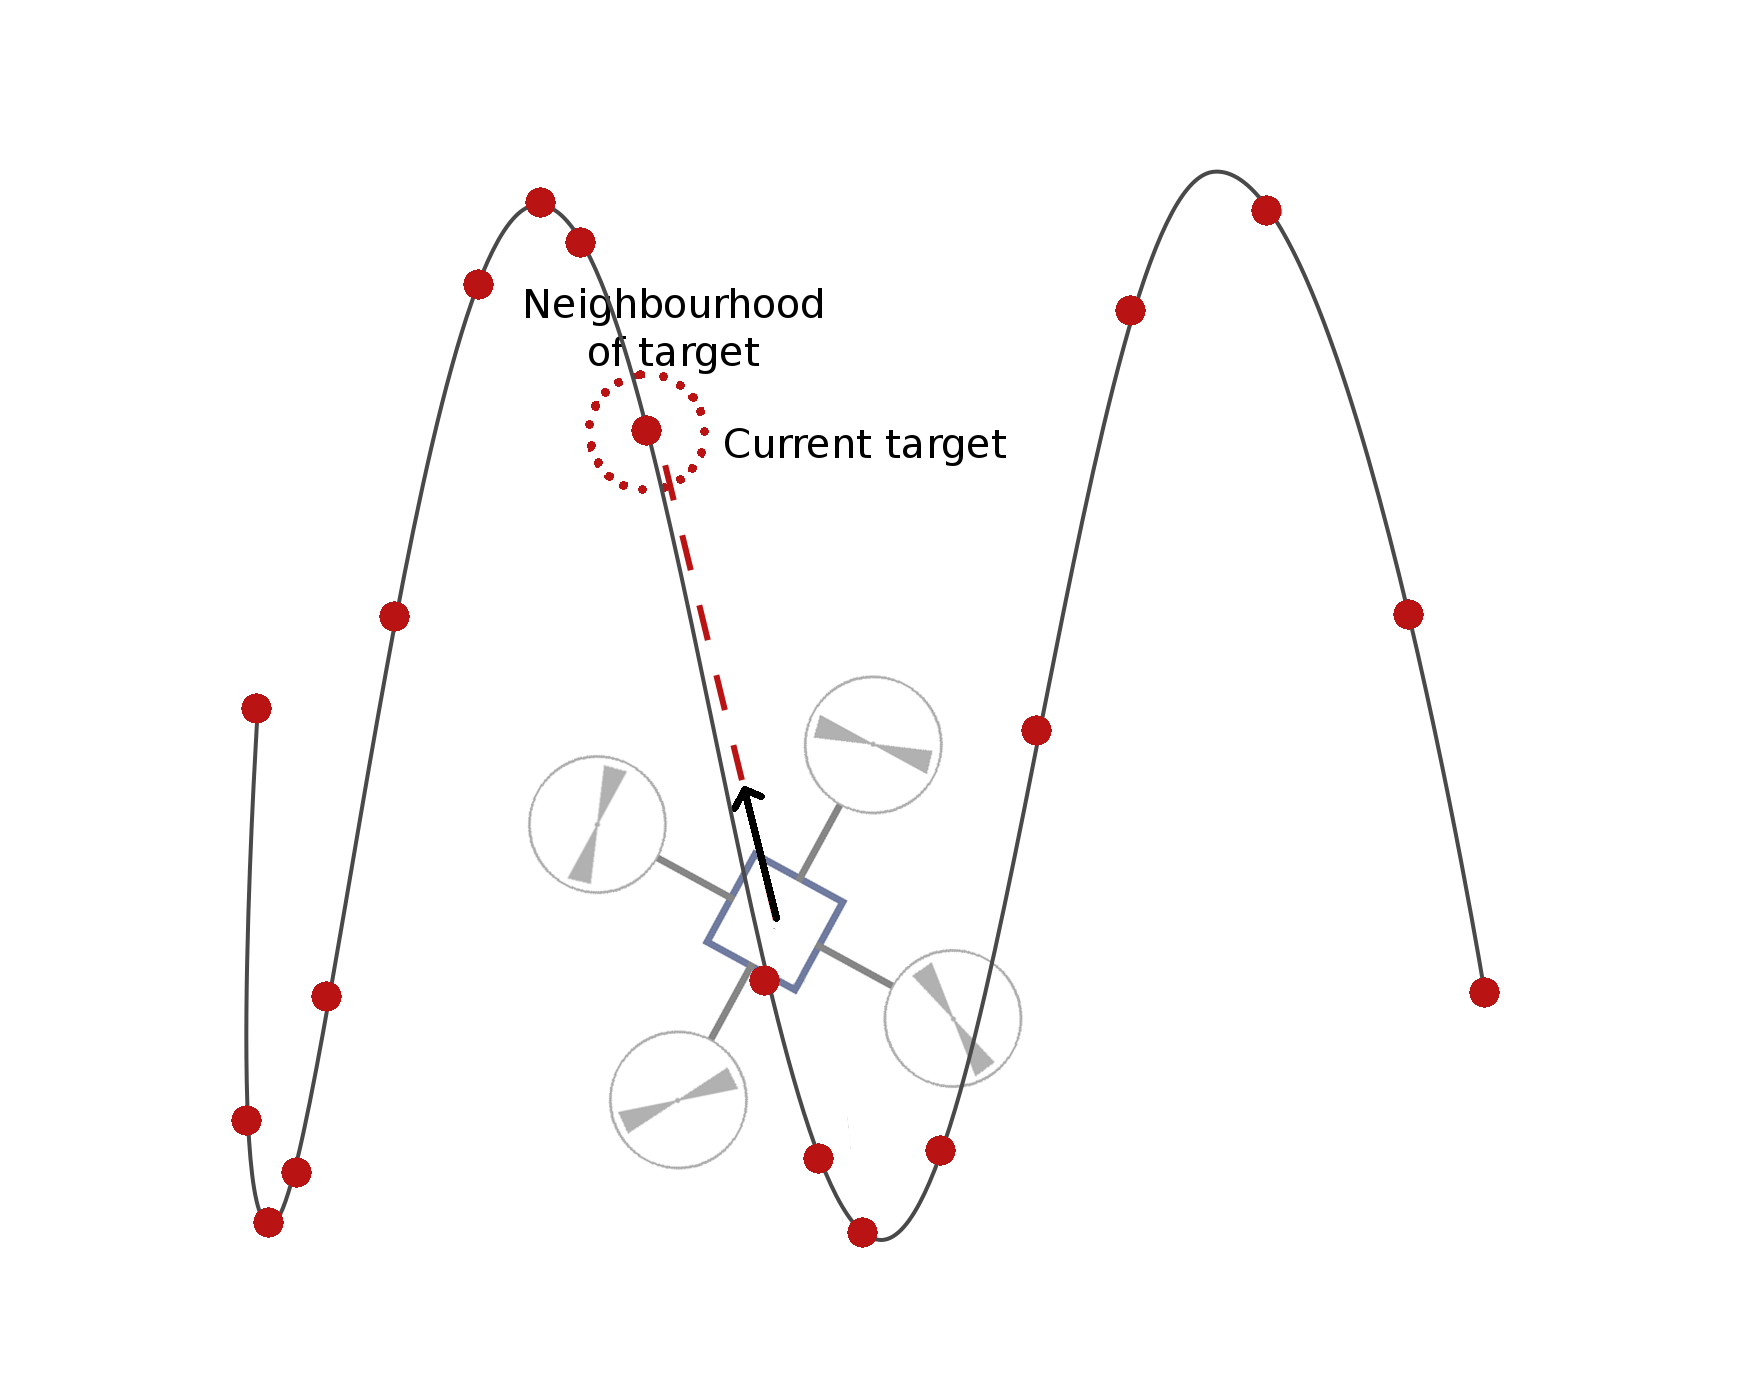
\includegraphics[width=0.6\textwidth]{checkpoint.png}
    \caption{Schematic of the checkpoint technique showing the quad-rotor and the set of checkpoints for this trajectory.}
\end{figure}

\begin{figure}[H]
  \centering
  \begin{subfigure}[t]{0.45\textwidth}
    \centering
      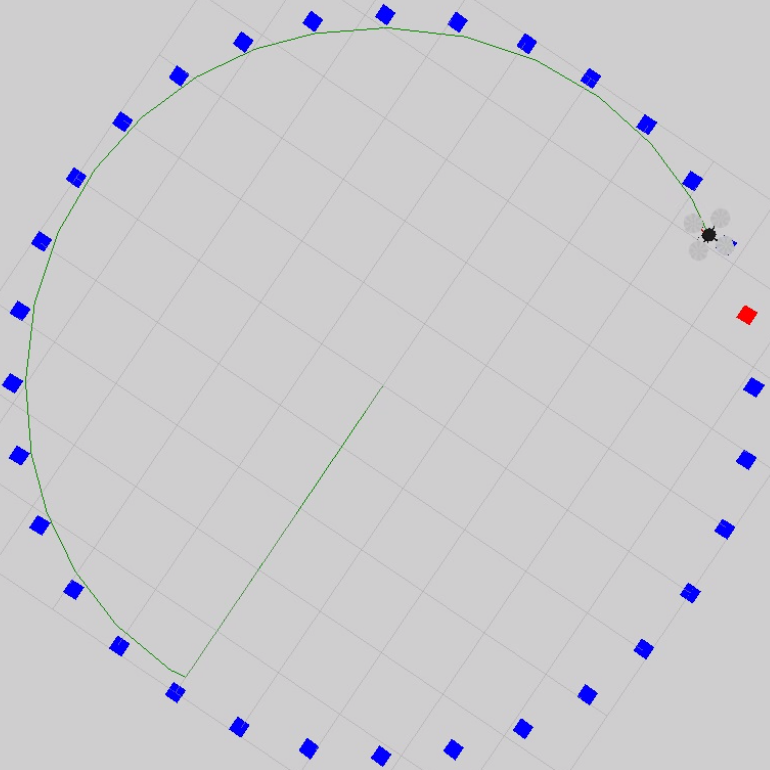
\includegraphics[width=\textwidth]{checkpoint_circle.png}
      \caption{With no stochasticity}
  \end{subfigure}
  \begin{subfigure}[t]{0.45\textwidth}
    \centering
      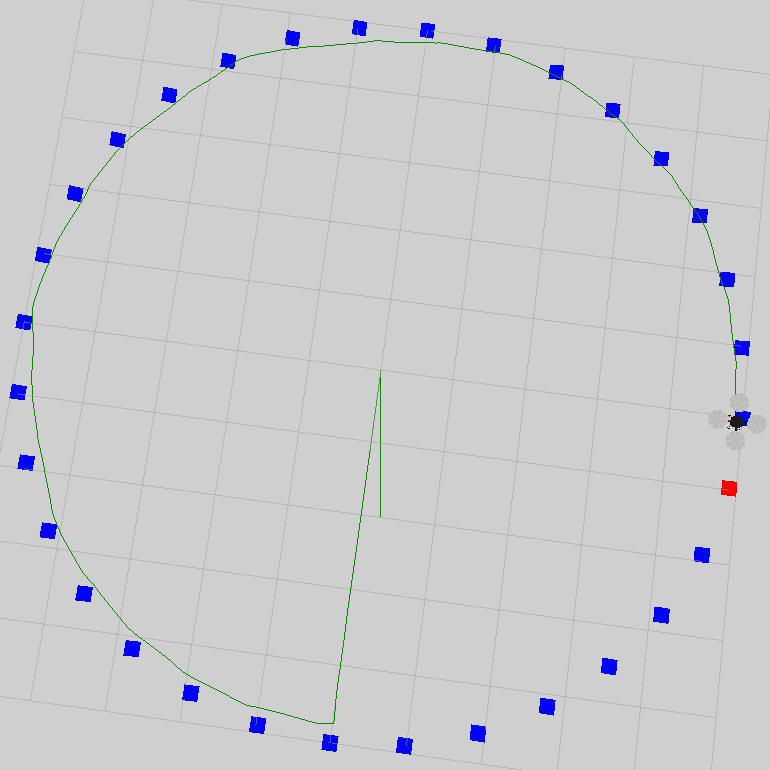
\includegraphics[width=\textwidth]{checkpoint_circle_wind.png}
      \caption{With large stochasticity - wind with uniform sum distribution limited to $5 m/s$}
  \end{subfigure}
  \caption{Quad-rotor simulation moving in a circular trajectory with the checkpoint technique. The red marker denotes the current targetted checkpoint and the blue markers are all the checkpoints in the trajectory.}
\end{figure}

\subsection{Jerky trajectories}
The underlying policy that is being used is the position control. So the quad-rotor thinks that it should stop at the next checkpoint because it has reached the target. Hence, it decelerates when it is in the checkpoint's vicinity. This causes the trajectory to be a little jerky adding excessive noise near the checkpoints.

Although the trajectory is jerky near the checkpoint, the trajectory followed by the quad-rotor will be piecewise smooth. Between checkpoints, the trajectory is interpolated as a smooth straight line. If the ceckpoints are further apart, the jerks will be fewer but the trajectory would lose definition (i.e. it would be an approximate of the original one). Hence, there is a tradeoff involved.

Also, the $\epsilon_i$ which is used to check whether the checkpoint was passed is a hard bound. For example, if the quad-rotor or payload is a little outside this boundary, the checkpoint is not passed. This makes things a little confusing, because a small margin of error could disrupt the whole trajectory. A possible method of fixing this fallacy is to use the velocity and judge whether the quad-rotor will be moving away from the trajectory or towards and set the bound based on this. This uses the intuitive understanding that the quad-rotor will in the future be on the right track or not.

Another possible solution for $\epsilon_i$ is to use fuzzy concepts to make the bound soft. The history of the trajectory can be used to compute how well the quad-rotor's current target helps to maintain this trajectory and how well changing the checkpoint will maintain the trajectory. This would give a metric to compare the two scenarios. "How well" a trajectory is maintained would need to be defined mathematically, which can be done by checking the smallest distance to the trajectory.

\subsection{Generating checkpoints}
There is no direct method to generate checkpoints. It is important that checkpoints are chosed with an appropriate distance between them. Intuitively, in a smooth part of the trajectory fewer checkpoints would be needed needed. But near a sharp turn, more checkpoints would be required so as to decelerate appropriately and make a fine turn. The checkpoints could be decided based on the derivative of the trajectory itself.

Other than this, consider plotting the trajectory using a software like Inkscape which makes an SVG representation. Vector graphics can define trajectories accurately as they have continuous paths as well as directed paths. Adobe's Snap \footnote{http://snapsvg.io/} can then be used to generate checkpoints in a smart way to reduce metrics like area error and deviation but with constraints like number of points imposed. This wouldn't take into account the deceleration and the speed control though. Snap can even help to animate the trajectory in a browser to visualize the path. Note that Snap is restricted to 2D cvg files, and cannot handle 3D at the time of writing.

\subsection{Retracing paths}
If a checkpoint is missed due to control error in the trajectory, the quad-rotor would be forced to go backward and find this checkpoint. This is counter productive and may not be a good idea because it modifies the original structure of the trajectory that had to be traced.


\begin{figure}[H]
  \centering
    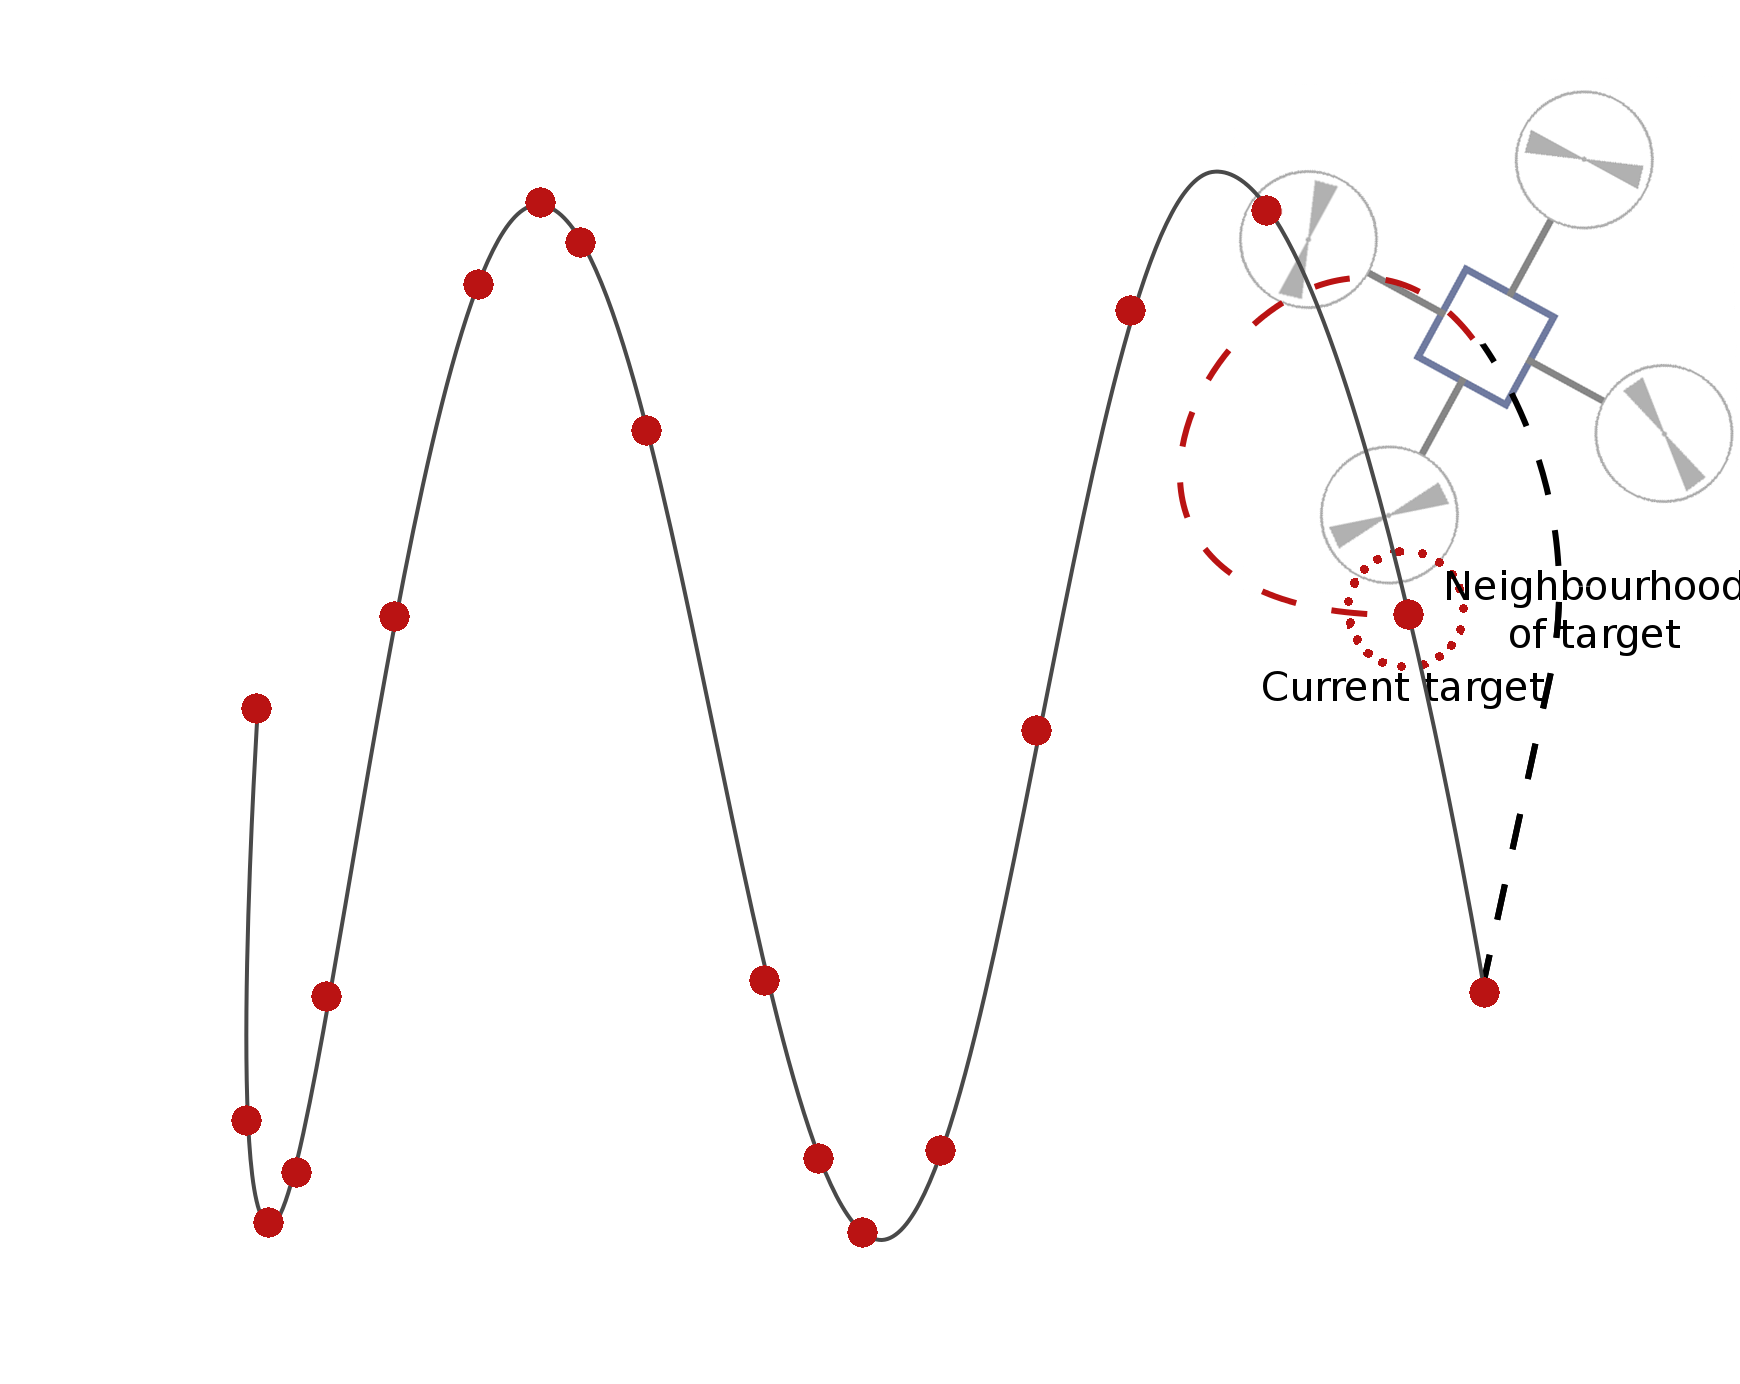
\includegraphics[width=0.6\textwidth]{checkpoint_con.png}
    \caption{Schematic of the checkpoint technique showing the quad-rotor's path if a checkpoint has been missed, the path of the quad-rotor is completely different from the original trajectory.}
\end{figure}

The Stanford Testbed of Autonomous Robocraft for Multi aent control (STARMAC) \cite{STARMAC} has done some work solving this problem by introducing the concept of waypoints to reduce retracing of paths which can occur in stochastic environmnets. This is a special case of checkpoints where the condition to pass is that the quad-rotor or payload passes the plane defined by the normal to the trajectory at this point. The quad-rotor or payload can also be restricted to pass through a specific patch in the plane. Also, this allows bounds to be set on the frame of the expected position rather than the absolute $(x, y, z)$ directions.

\begin{figure}[H]
  \centering
    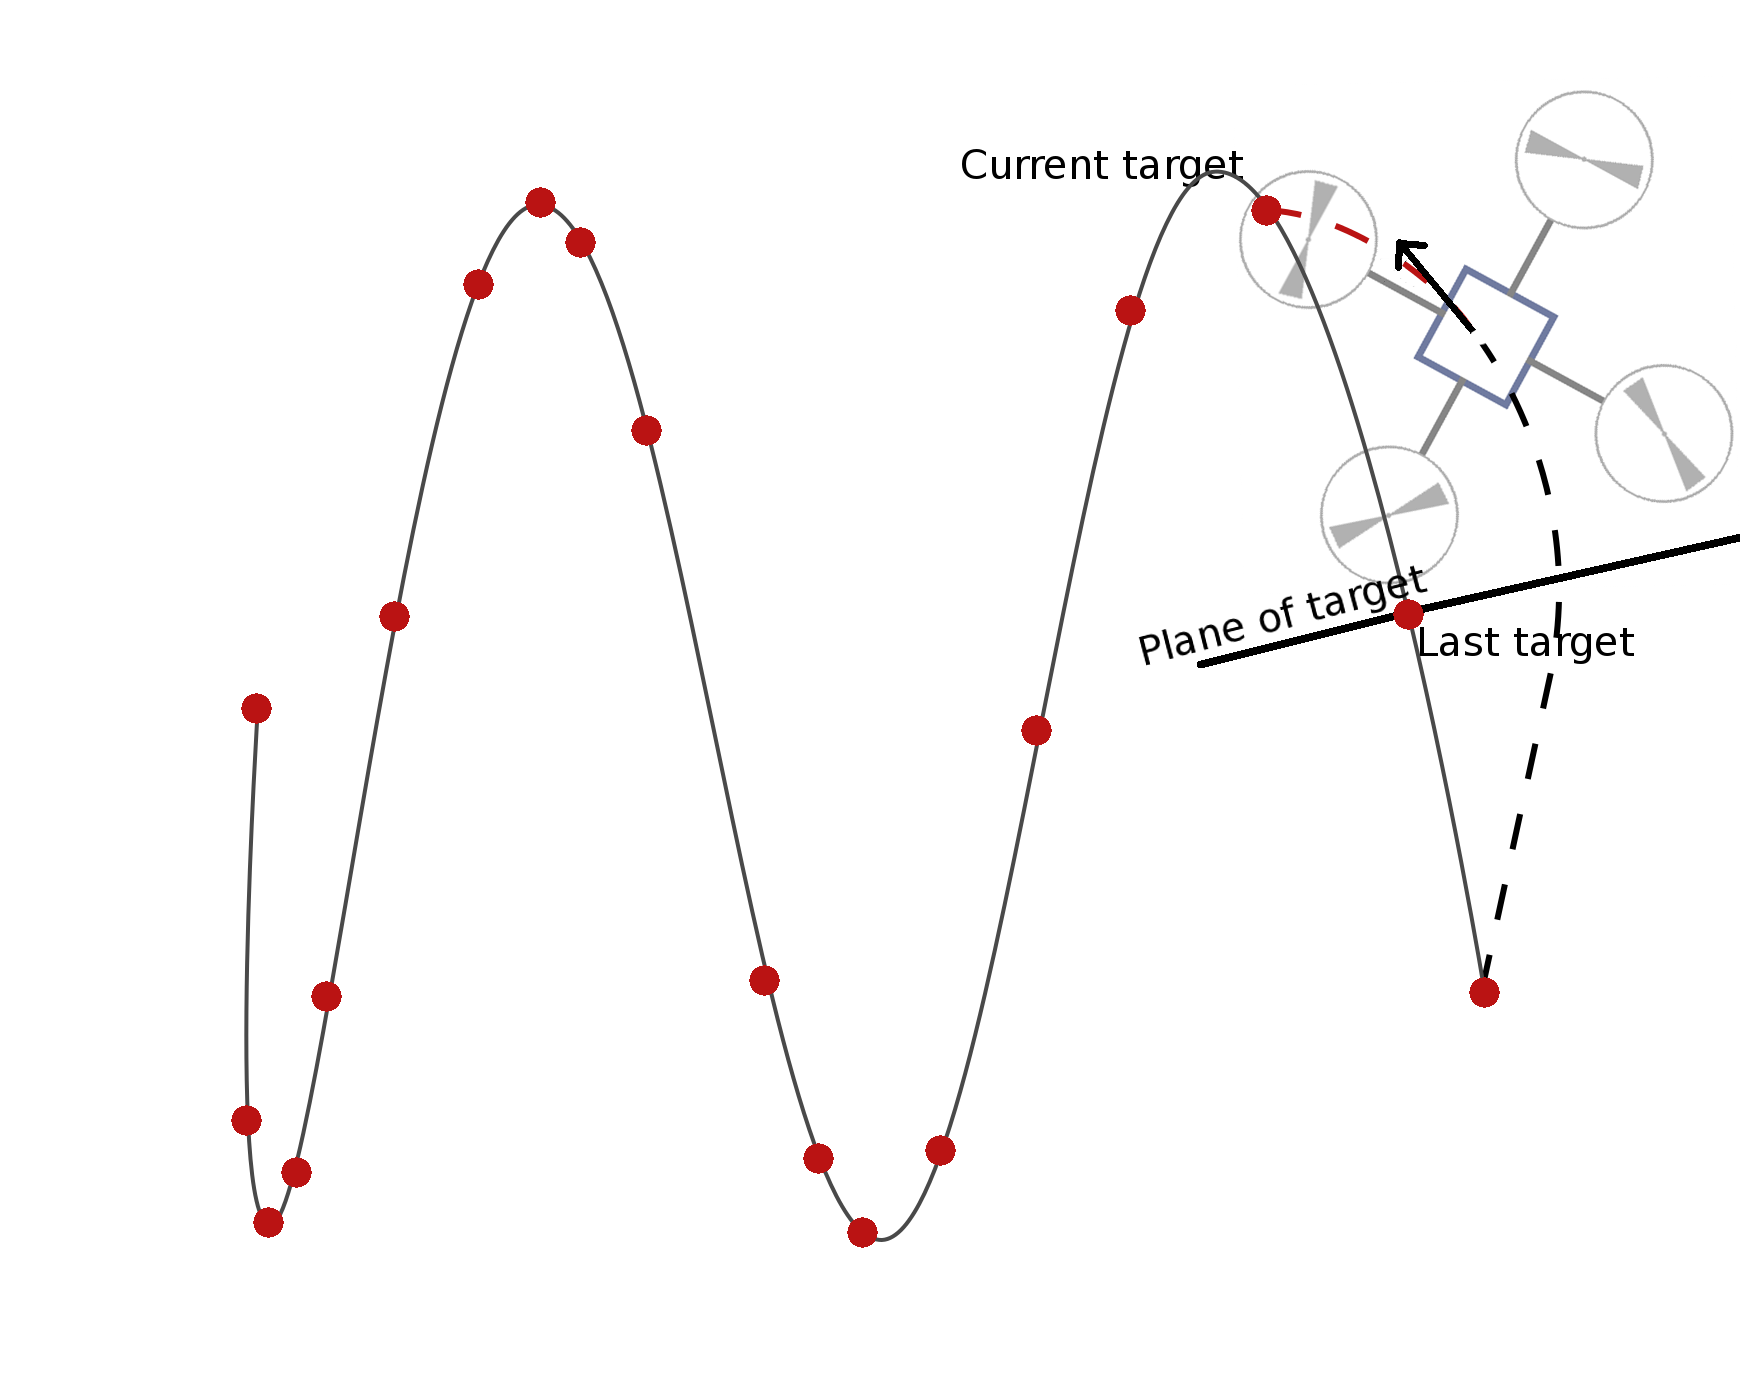
\includegraphics[width=0.6\textwidth]{waypoint.png}
    \caption{Schematic of the waypoint technique showing the quad-rotor and the set of waypoints for this trajectory. The plane of the last target is shown where the quad-rotor did not go through an $\epsilon$ neighbourhood of the waypoint, but passed the plane.}
\end{figure}

Because the quad-rotor needs to simply pass the plane of the waypoint, even if the control is not good at certain areas, it does not change the original structure of the trajectory. This comes at the cost that the error in this direction could increase over time. However, that would not happen experimentally as the quad-rotor policy would not allow an unbounded error unless there is a flaw in the controller.

\section{Pursuit based trajectory control}

In pursuit, the complete trajectory function with time is known. Here, the target of the quad-rotor is changed at every step to be the expected position after a certain time. Hence, the quad-rotor or payload tries to pursue the trajectory where the target has a time lead.

\begin{figure}[H]
  \centering
    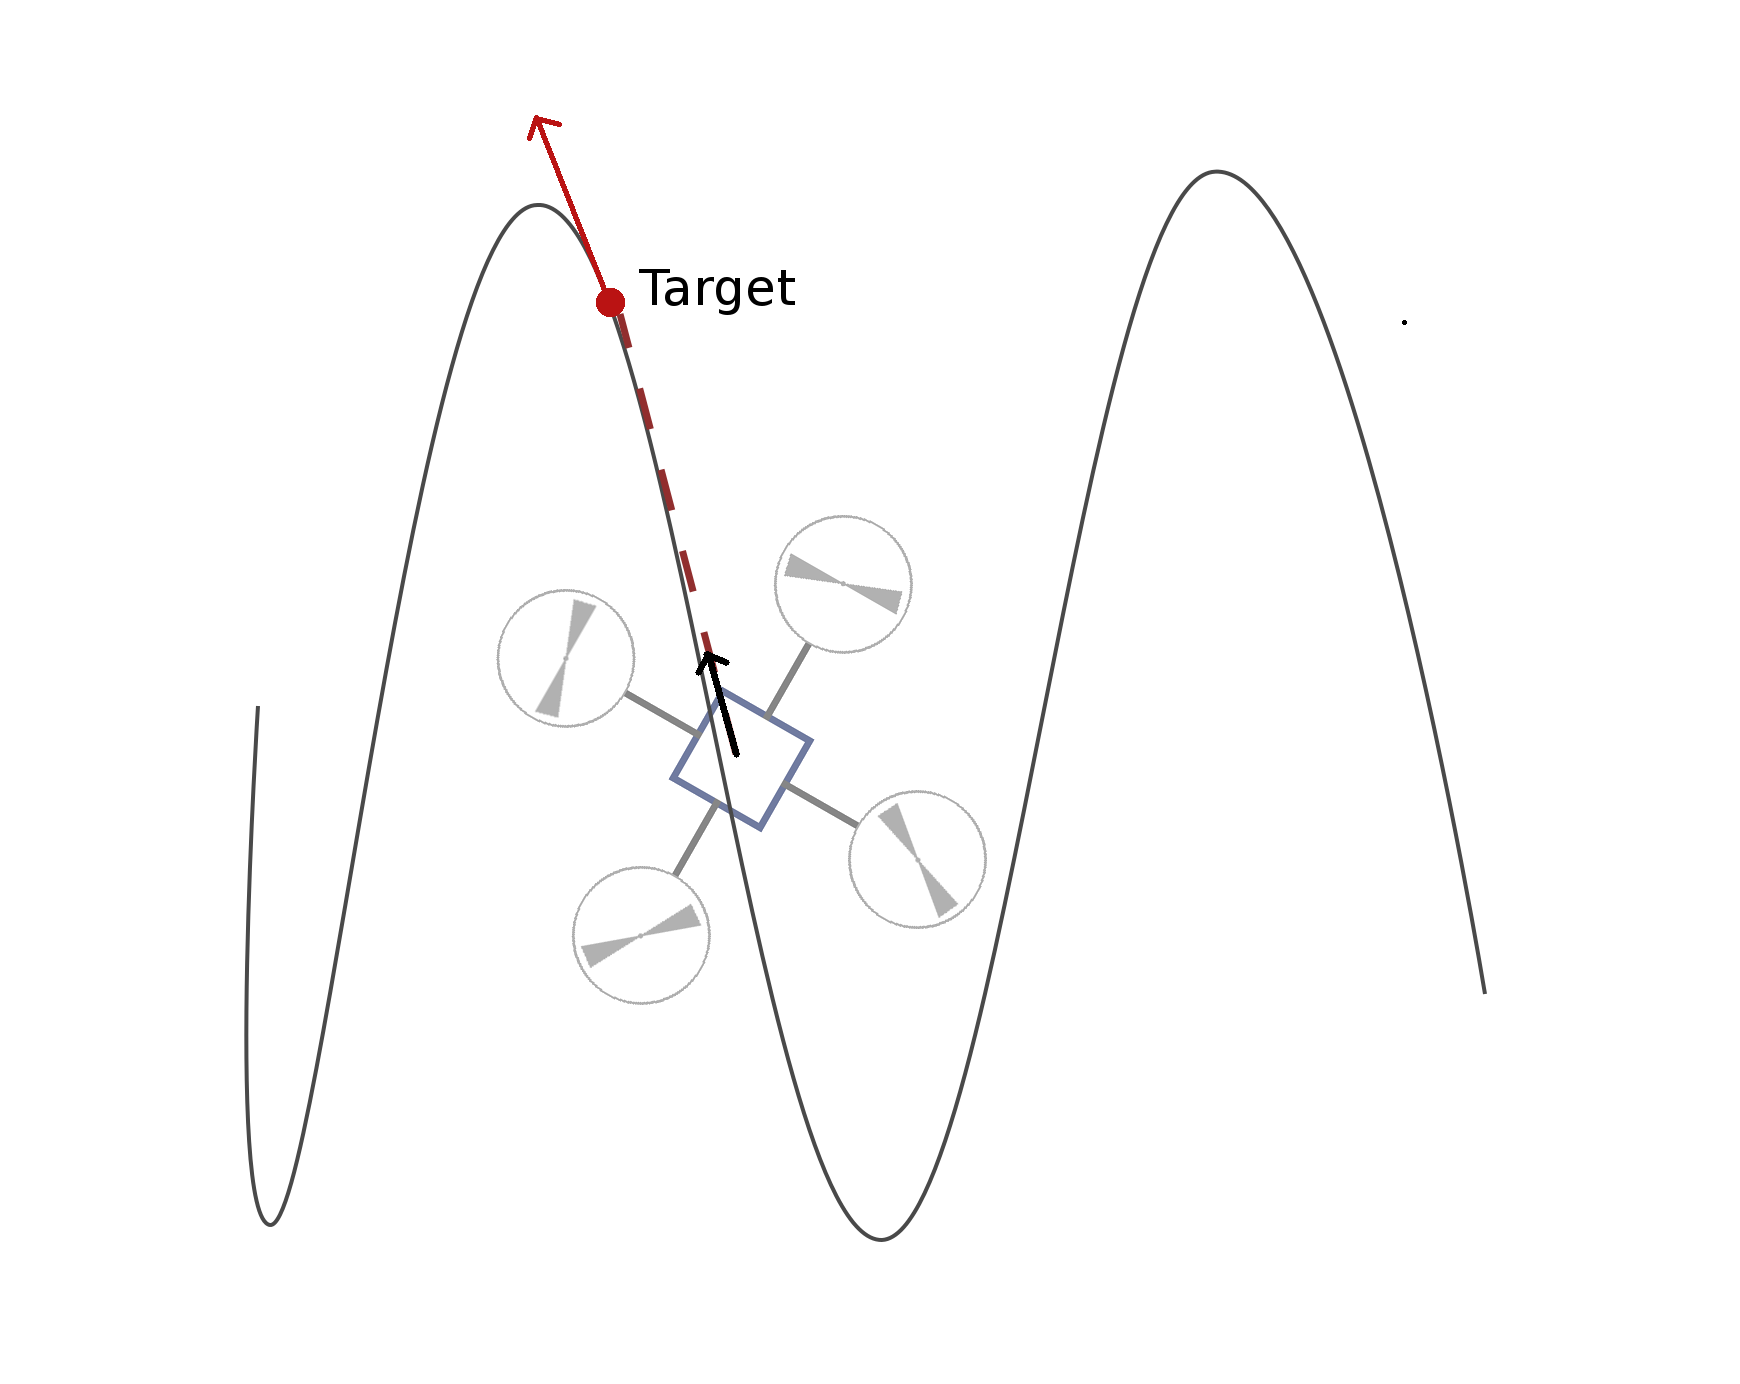
\includegraphics[width=0.6\textwidth]{pursuit.png}
    \caption{Schematic of the pursuit technique showing the quad-rotor and the leading target. The velocities of the target and the quad-rotor indicate how they will move next.}
\end{figure}

\begin{figure}[H]
  \centering
  \begin{subfigure}[t]{0.45\textwidth}
    \centering
      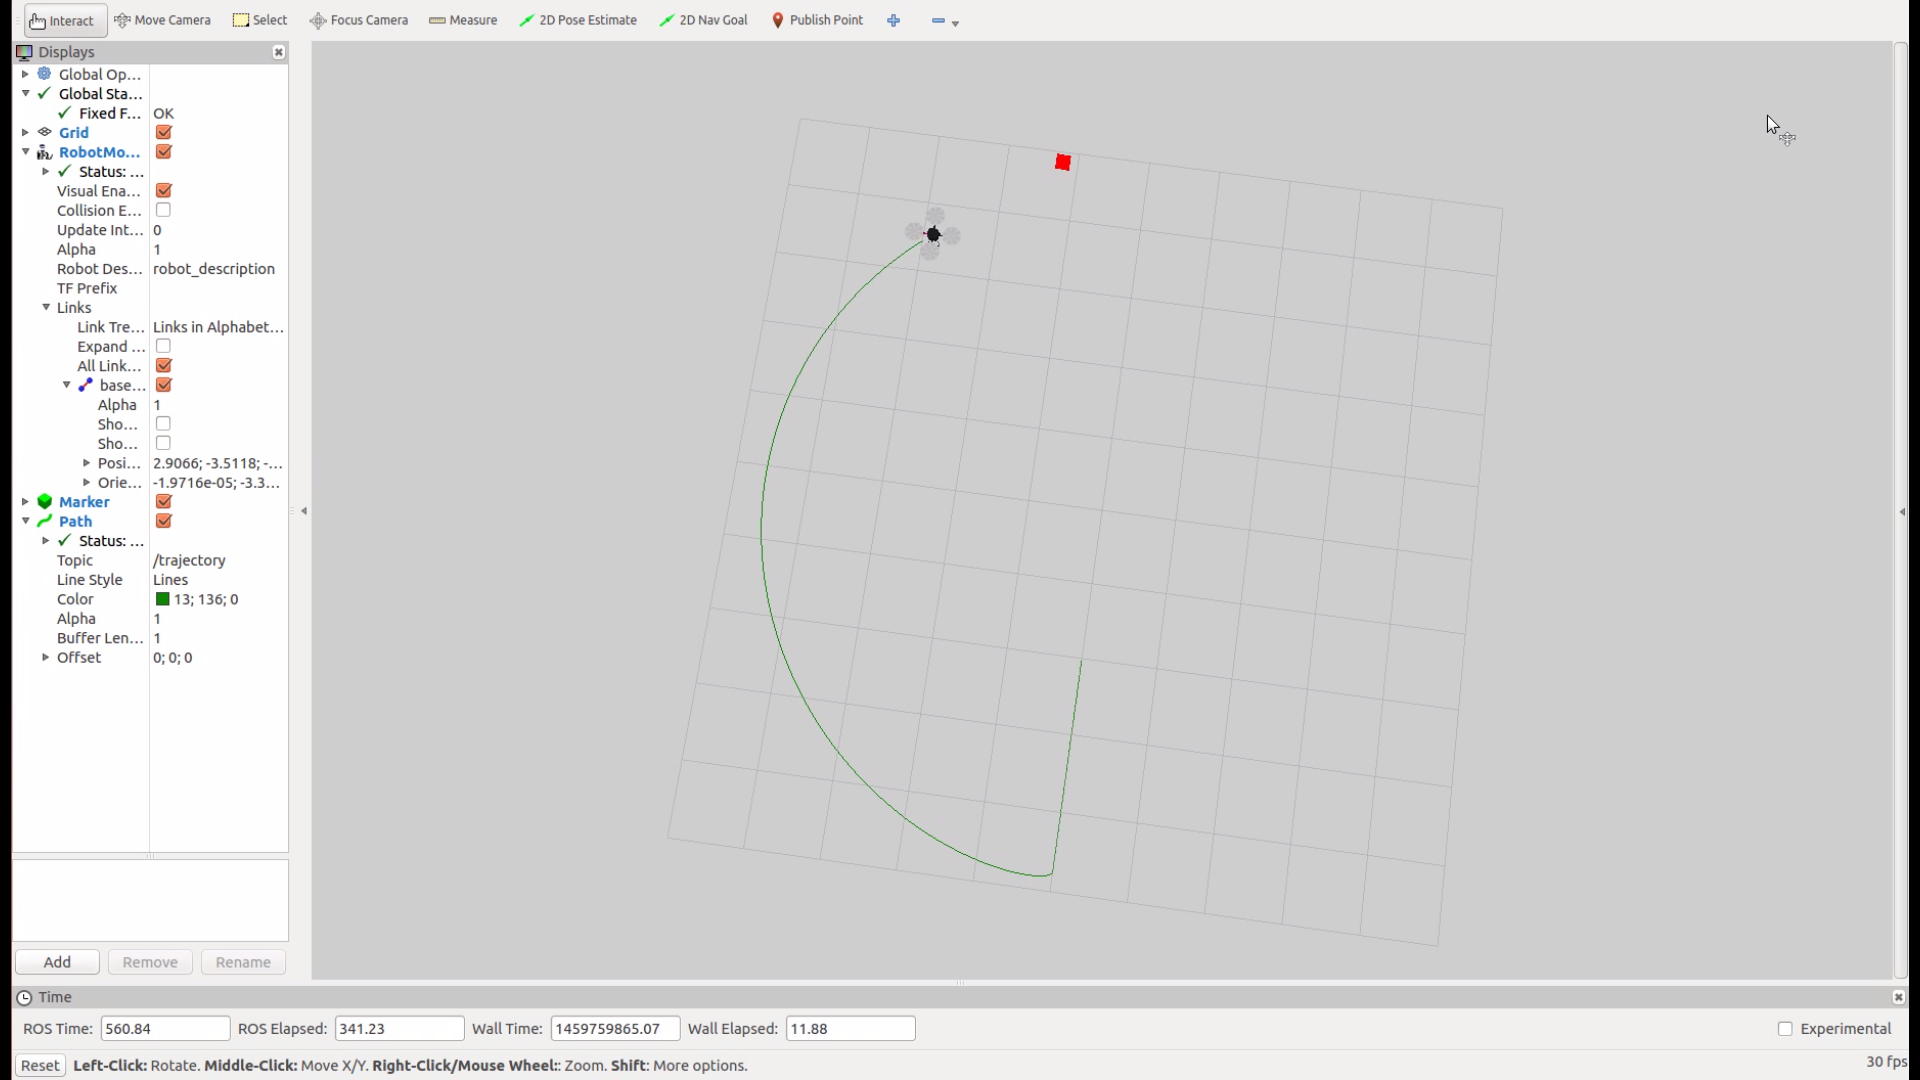
\includegraphics[width=\textwidth]{pursuit_circle.png}
      \caption{With no stochasticity}
  \end{subfigure}
  \begin{subfigure}[t]{0.45\textwidth}
    \centering
      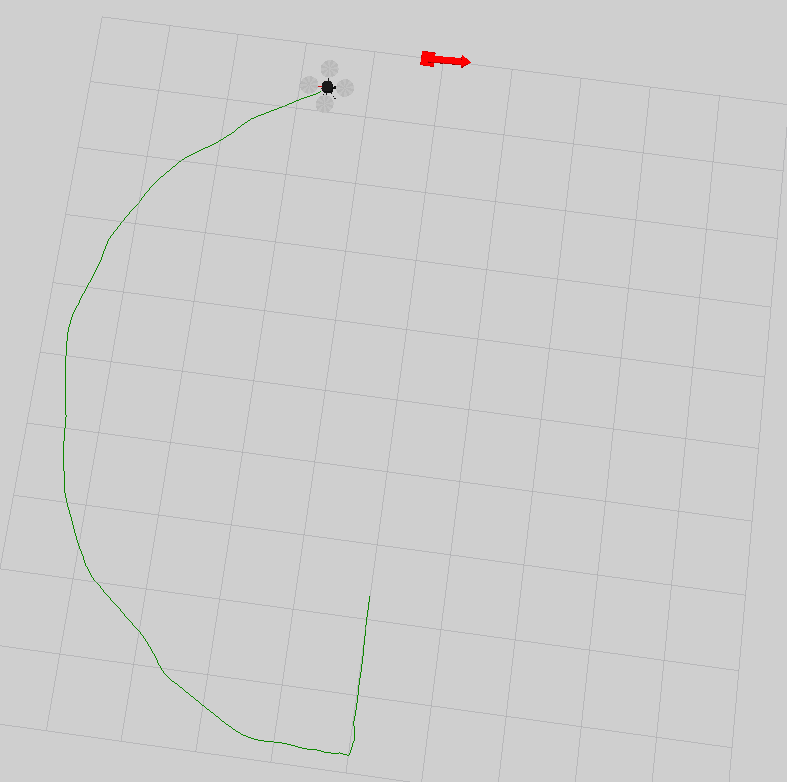
\includegraphics[width=\textwidth]{pursuit_circle_wind.png}
      \caption{With large stochasticity - wind with uniform sum distribution limited to $5 m/s$}
  \end{subfigure}
  \caption{Quad-rotor simulation moving in a circular trajectory with the pursuit technique. The red marker and arrow denote the current position and velocity of the target.}
\end{figure}

\subsection{Accumulated error}
A continuous pursuit would also mean that the target is never reached (as the target moves). This means that if there is an initial error when the trajectory began or if there is anomalous behaviour due to stochasticity at some points, the agent may never recover. These would result in a completely different trajectory from the planned trajectory because there is no feedback to the trajectory generator. Hence, this is not suitable for stochastic problems where a gust of wind could blow the quad-rotor away completely.

For environments where the stochasticity is not much this is a great value add though, as it gives an extremely smooth trajectory. If there is a "slowness" factor incorporated in the trajectory which makes the target move slower if the quad-rotor lags behind too much, this would help in resolving this issue.

\subsection{Lead time}
The amount of time by which the trajectory is leading will affect the actual trajectory the quad-rotor will fly. This may depend on trajectory to trajectory, for example a square would need a small lead time whereas a circle or oval would work well with a larger one in comparison. A straight line can have a large lead time.

\begin{figure}[H]
  \centering
    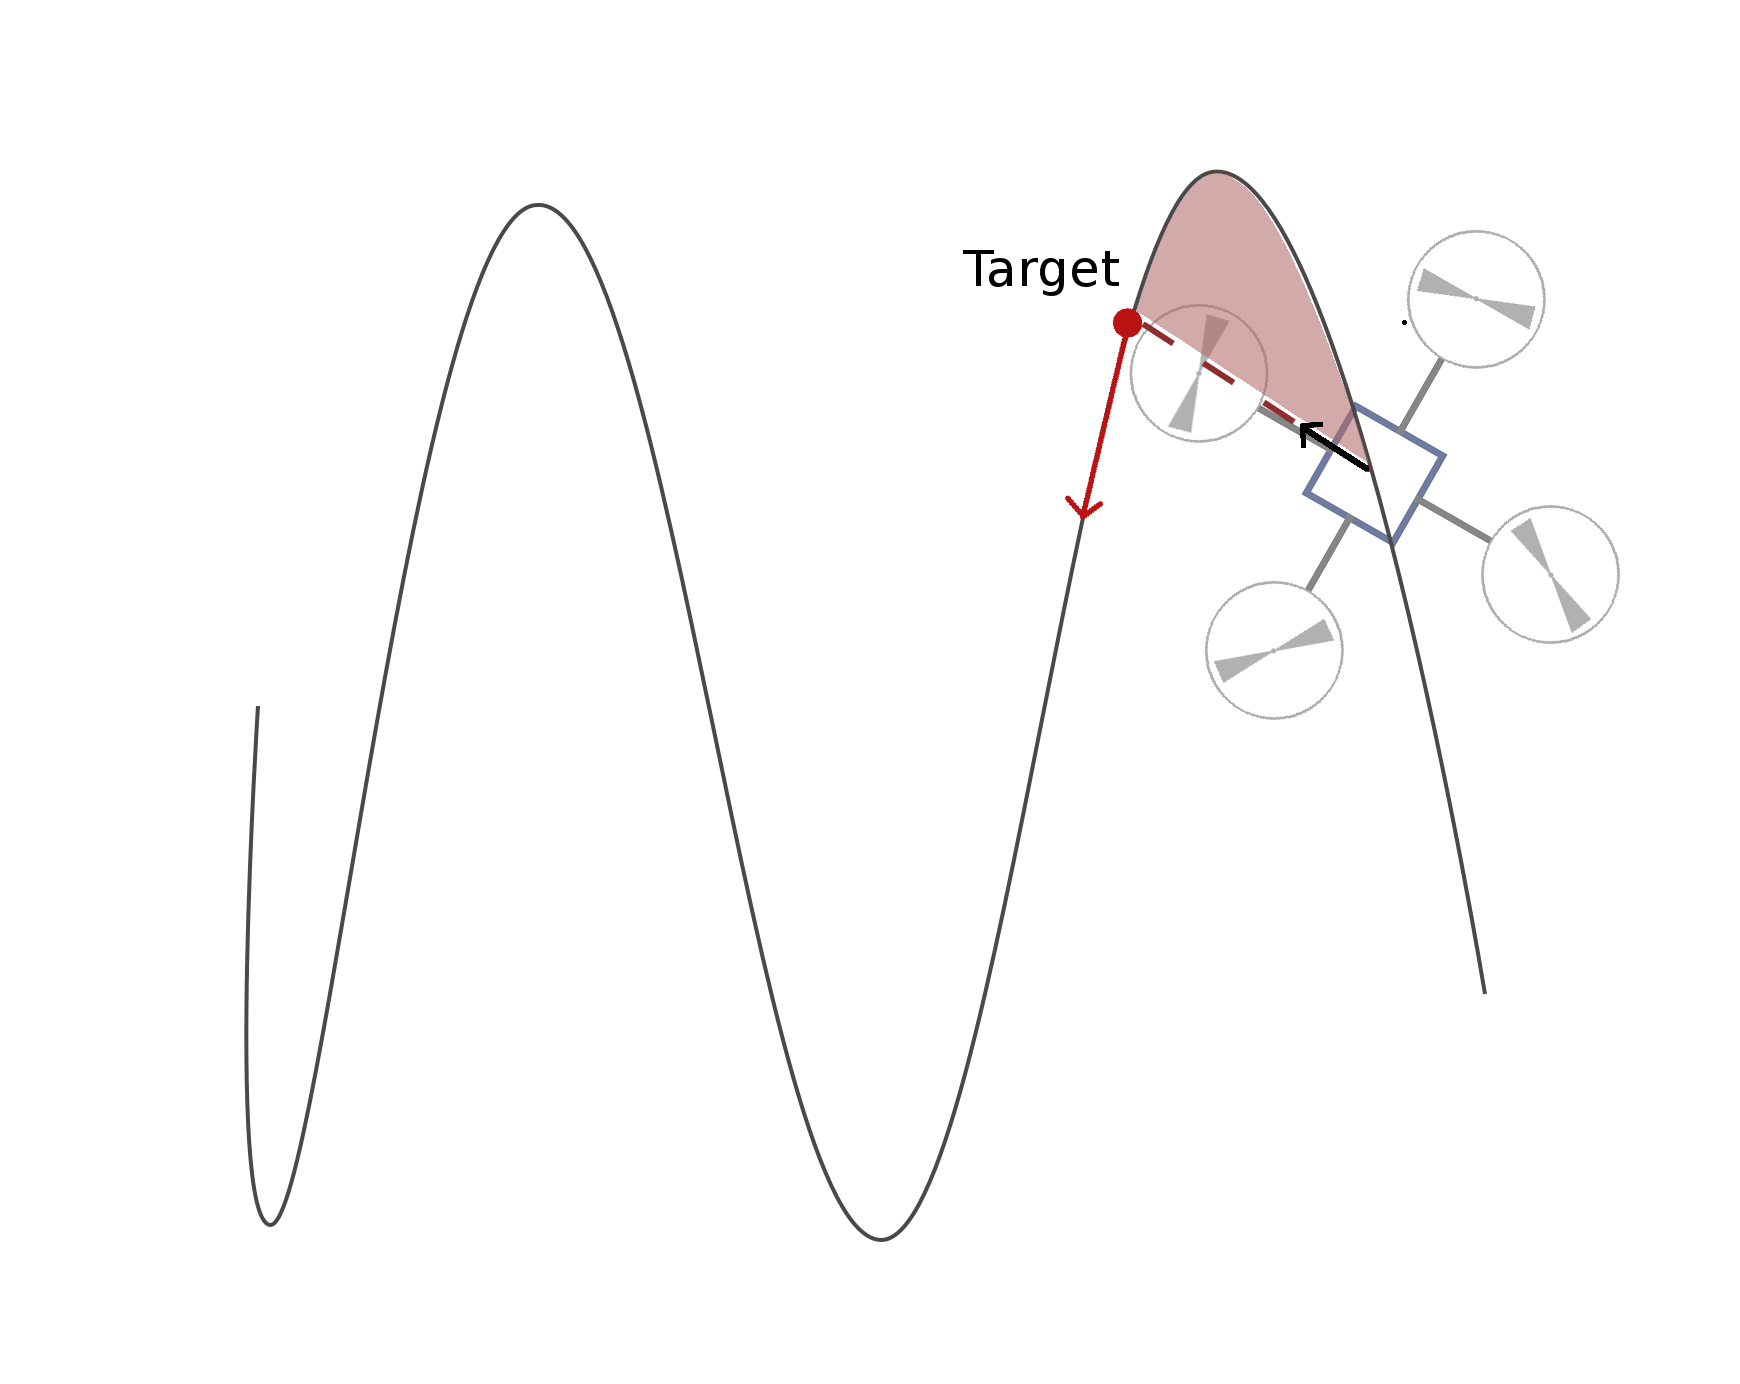
\includegraphics[width=0.6\textwidth]{pursuit_con.png}
    \caption{Schematic of the pursuit technique showing the quad-rotor and the leading target in a case where a portion of the trajectory is ignored because the target is leading by a large amount.}
\end{figure}

A constant leading time may be harmful because the leading time would depend on the trajectory itself. For example, a sharp corner would need a small leading time while a smooth trajectory would not need a small leading time. If the leading time is set to be too small, the quad-rotor would move very slowly as it assumes the target is close by.

Due to the fact that the target trajectory is continuous and changes with every time step, the trajectory generated by this method is extremely smooth. The major issue of this method is that there is no feedback from the quad-rotor to the trajectory generator, which makes it impossible for the quad-rotor to recover if it deviates from the path.

\section{Comparison of trajectory techniques}

\subsection{Accuracy}
The accuracy of the trajectory being followed is an important aspect which needs to be considered. To compare accuracy, it needs to be quantified. One method of computing accuracy is to find the deviation of the actual position of the quad-rotor to the expected position at every time.

Consider the experiment of a circular trajectory with a radius $r$ centered at $(0,0,0)$ on the XY plane. The expected trajectory would make the quad-rotor be at a distance of $r$ at all times from the center. The distance of the quad-rotor from the origin is measured and compared to the radius of the circle being followed.

\begin{figure}[H]
  \centering
    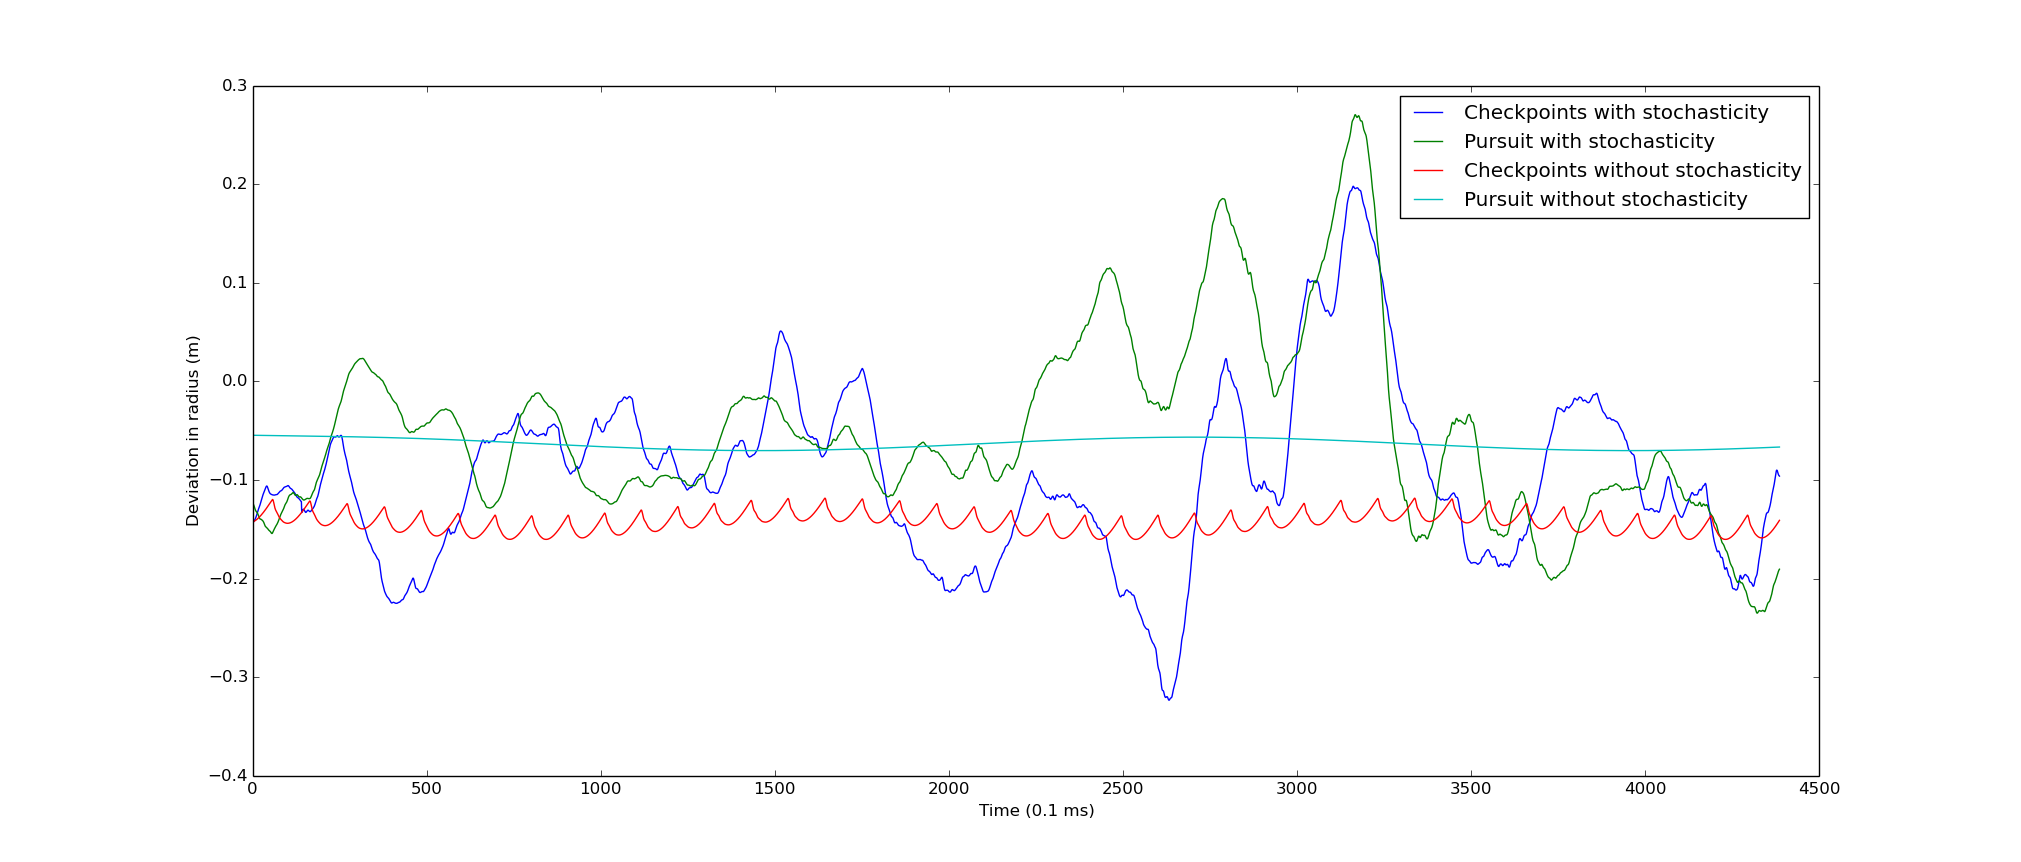
\includegraphics[width=\textwidth]{comparison_accuracy.png}
    \caption{Comparison of accuracy in trajectory control techniques following a 2D circular path with and without wind.}
    \label{fig:TrajectoryComparison}
\end{figure}

\subsection{Smoothness of the trajectory}
There are two metrics to consider smoothness. One is the smoothness of the spatial function of the trajectory. For example, whether the trajectory has extra edges while the original trajectory does not. The other metric to consider smoothness is related to time, the smoothness of the agent's motion on the trajectory and whether the velocity and acceleration is the expected value.

Once again consider the experiment of a circular trajectory with a radius $r$ centered at $(0,0,0)$ on the XY plane. Plotting the deviation from the expected radius over time, and finding the peaks gives a method of computing smoothness. This can be seen in Figure \ref{fig:TrajectoryComparison}. The plot for the checkpoint based method is not smooth as it has a large number of steep peaks when compared to the rest.

The smoothness of velocity method to measure smoothness can also be found in the circular trajectory experiment. Here, the magnitude of the velocity (speed) is plotted and the variation is analyzed. It is seen that the checkpoints method decelerates the agent when the checkpoint is close by and accelerates after it passes the checkpoint. This is not seen in pursuit as the target there is at a nearly constant distance from the agent based on the time lead.

\begin{figure}[H]
  \centering
    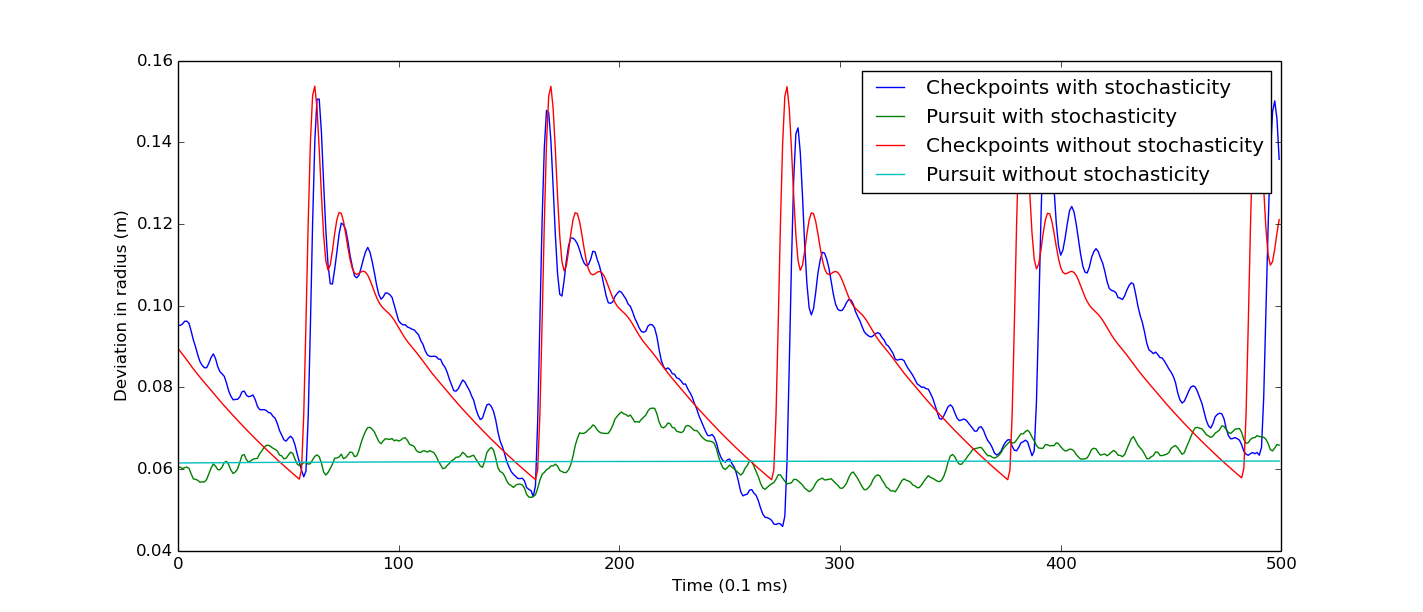
\includegraphics[width=\textwidth]{comparison_velocity.png}
    \caption{Comparison of speed in trajectory control techniques following a 2D circular path with and without wind.}
\end{figure}

\subsection{Speed control}
The speed of the quad-rotor is not easy to control in either of the methods. This is because the underlying policy is that for hovering, and trajectories are created by truncating the hovering policy in quick succession.

In the checkpoint method, the quad-rotor attempts to decelerate as the target is nearly reached. This makes the speed of the quad-rotor vary excessively. Although there is some notion that the checkpoint is only required for turns, where the quad-rotor would need to slow down to avoid over shooting, this is not very intuitive nor rigorously controllable.

In the pursuit method, the lead that the target has would determine the speed, and hence the further away the leading target is, the faster the quad-rotor would be. This is because the quad-rotor would decelerate as it approaches the target - because the PEGASUS model has been learnt for a target velocity of zero. Although there is some notion that the faster the target is, the faster the quad-rotor will be this is not easy to control.

\section{Unstable trajectories}
Note that the reward function and policy class described in the PEGASUS method above is incapable of performing a flip as it is only meant for stable states. For unstable trajectories, apprenticeship learning is useful. Unstable trajectories include things like in place flips, loops, and hurricanes.

As mentioned earlier, apprenticeship learning requires two steps:
\begin{itemize}
\item{Dynamic Time warping}
\item{EM based kalman filter smoothening}
\end{itemize}

\todo{Elaborate on how we don't use Kalman filter}

\todo{Elaborate on how DTW was used}

By trial and error, slantedband windowing was the best suited for our use case the best.

%%%%%%%%%%%%%%%%%%%%%%%%%%%%%%%%%%%%%%%%%%%%%%%%%%%%%%%%%%%%
% Bibliography.

\begin{singlespace}
  \pagebreak
  \clearpage
  \phantomsection
  \addcontentsline{toc}{chapter}{References}
  \bibliography{refs}
\end{singlespace}

\end{document}
